% DEADLINE: 12 NOON, FRIDAY, 21ST AUGUST 2015
%
% The project is only assessed on the basis of a final written
% thesis. Additional material, such as the code you submit, may be taken
% into account in case of doubt, but you should make sure that all the
% work you have done is carefully described in the thesis. Theses will
% typically conform to the following format:
%
% * The length should be 40 -- 70 pages in total and no shorter than 35
%   pages.
%
% * Title page with abstract.
%
% * Introduction: an introduction to the document, clearing stating
%   the hypothesis or objective of the project, motivation for the work
%   and the results achieved. The structure of the remainder of the
%   document should also be outlined.
%
% * Background: background to the project, previous work, exposition of
%   relevant literature, setting of the work in the proper context. This
%   should contain sufficient information to allow the reader to
%   appreciate the contribution you have made.
%
% * Description of the work undertaken: this may be divided into
%   chapters describing the conceptual design work and the actual
%   implementation separately. Any problems or difficulties and the
%   suggested solutions should be mentioned. Alternative solutions and
%   their evaluation should also be included.
%
% * Analysis or Evaluation: results and their critical analysis should
%   be reported, whether the results conform to expectations or
%   otherwise and how they compare with other related work. Where
%   appropriate evaluation of the work against the original objectives
%   should be presented.
%
% * Conclusion: concluding remarks and observations, unsolved problems,
%   suggestions for further work.  Bibliography.
%
% In addition, the thesis must be accompanied by a statement declaring
% that the student has read and understood the University's plagiarism
% guidelines. Students should budget at least six weeks for the final
% thesis writing-up phase. Where appropriate the thesis may additionally
% contain appendices in which relevant program listings, experimental
% data, circuit diagrams, formal proofs, etc. may be included. However,
% students should keep in mind that they are marked on the quality of
% the thesis, not its length. The thesis must be word-processed using
% either LaTeX or a system with similar capabilities. The LaTeX thesis
% template can be found via the local packages web page. You don't have
% to use these packages, but your thesis must match the style (i.e.,
% font size, text width etc) shown in the sample output for an
% Informatics thesis. Technical problems during project work are only
% considered for resources we provide; no technical support,
% compensation for lost data, extensions for time lost due to technical
% problems with external hard- and software as provided will be given,
% except where this is explicitly stated as part of a project
% specification and adequately resourced at the start of the project.


%%%%%%%%%%%%%%%%%%%%%%
%% Document details %%
%%%%%%%%%%%%%%%%%%%%%%

% Author
\author{Chris Cummins}

% Date (Month Year)
\date{August 2014}

% Paper title
\title{Dynamic Autotuning\\of Algorithmic Skeletons}

% Subtitle
\newcommand{\subtitle}{MSc by Research Thesis}

% Degree title
\newcommand{\degreeTitle}{MSc by Research\\ Pervasive Parallelism}

% Institution
\newcommand{\institution}{School of Informatics,\\
  The University of Edinburgh}

%%%%%%%%%%%%%%%%%%%%%%%%%
%% Document and Layout %%
%%%%%%%%%%%%%%%%%%%%%%%%%

% Fix for multiple "No room for a new \dimen" errors.
%
% See: http://tex.stackexchange.com/questions/38607/no-room-for-a-new-dimen
%
\usepackage{etex}

\usepackage{booktabs}

\usepackage[utf8]{inputenc}

% Make internal macro definitions accessible,
% e.g. \@title, \@date \@author.
\makeatletter

% Multi-column support.
\usepackage{multicol}

% A useful package which includes macros like \ifdef{}{}{}:
%
\usepackage{etoolbox}

% Uncomment the following line to remove column separation:
%
%\setlength{\columnsep}{5mm}


% Set chapter and section numbering depth:
%
\setcounter{secnumdepth}{2}


%%%%%%%%%%%%%%%%%%%%%%%%%%%%%%%%%
%% Bibliography and Appendices %%
%%%%%%%%%%%%%%%%%%%%%%%%%%%%%%%%%
\usepackage[%
    backend=biber,
    style=numeric-comp,  % numerical-compressed
    sorting=none,        % nty,nyt,nyvt,anyt,anyvt,ynt,ydnt,none
    sortcites=true,      % sort \cite{b a d c}: true,false
    block=none,          % space between blocks: none,space,par,nbpar,ragged
    indexing=false,      % indexing options: true,false,cite,bib
    citereset=none,      % don't reset cites
    isbn=false,          % print ISBN?
    url=false,           % print URL?
    doi=false,           % print DOI?
    natbib=true,         % natbib compatability
  ]{biblatex}

% Reduce the font size of the bibliography:
% \renewcommand{\bibfont}{\normalfont\scriptsize}

% Determine which BibTeX file to use:
%
% If available, use my Mendeley BibTex library, located in the home
% directory. Note that this is a relative path and will break if
% either this file or the BibTex library are moved. If the library is
% not present, use the local refs.bib file.
\newcommand{\BibResourceGlobal}{../../../../library.bib}
\newcommand{\BibResourceLocal}{refs.bib}

\IfFileExists{\BibResourceGlobal}
  {\newcommand{\BibResource}{\BibResourceGlobal}}
  {\newcommand{\BibResource}{\BibResourceLocal}}

\addbibresource{\BibResource}

% Appendix package. Documentation:
%
%  http://mirror.ox.ac.uk/sites/ctan.org/macros/latex/contrib/appendix/appendix.pdf
%
% Package options:
%
% toc      - Put a header (e.g., `Appendices') into the Table of Contents
%            (the ToC) before listing the appendices. (This is done by
%            calling the \addappheadtotoc command.)
% page     - Puts a title (e.g., `Appendices') into the document at the
%            point where the appendices environment is begun. (This is
%            done by calling the \appendixpage command.)
% title    - Adds a name (e.g., `Appendix') before each appendix title in
%            the body of the document. The name is given by the value
%            of \appendixname. Note that this is the default behaviour
%            for classes that have chapters.
% titletoc - Adds a name (e.g., `Appendix') before each appendix listed
%            in the ToC. The name is given by the value
%            of \appendixname.
% header   - Adds a name (e.g., `Appendix') before each appendix in page
%            headers.  The name is given by the value
%            of \appendixname. Note that this is the default behaviour
%            for classes that have chapters.
\usepackage[title, titletoc]{appendix}


%%%%%%%%%%%%%%%%%%%%%%%%%%%%%%%%%%%%%
%% Figures, footnotes and listings %%
%%%%%%%%%%%%%%%%%%%%%%%%%%%%%%%%%%%%%

%\usepackage{float}
%\restylefloat{figure}

% Use bold ``(Figure|Table|Listing)'' caption text.
%\usepackage[margin=1cm]{caption}

% Set the font for captions.
%\renewcommand{\captionfont}{\footnotesize}
% Set the font for caption labels.
%\renewcommand{\captionlabelfont}{\footnotesize\bf}

% Use arabic numbers for footnote.
%\renewcommand{\thefootnote}{\arabic{footnote}}

% Ensure that footnotes always appear at the bottom of pages.
%\usepackage[bottom]{footmisc}

% Reset the footnote counter on every page.
%\usepackage{perpage}
%\MakePerPage{footnote}

% Pre-requisites for rendering upquotes in listings package.
\usepackage[T1]{fontenc}
\usepackage{lmodern}
\usepackage{textcomp}

% Pseudo-code listings.
\usepackage{algorithm}
\usepackage{algpseudocode}
\newcommand{\Break}{\State \textbf{break} }
\algblockdefx[Loop]{Loop}{EndLoop}[1][]{\textbf{Loop} #1}{\textbf{End
    Loop}}

\algrenewcommand\ALG@beginalgorithmic{\footnotesize}

% Code listings.
\usepackage{listings}

% Set \ttfamily to use courier fonts.
%
% See: http://tex.stackexchange.com/a/33686
%
\usepackage{courier}

\lstset{frame=bt,                    % Add top and bottom frame lines
        breaklines=true,             % Force line wrapping
        captionpos=b,                % Place caption below listing
        numbers=left,                % Add left-side line numbers
        basicstyle=\scriptsize\ttfamily, % Set font size and type
        showstringspaces=false,      % Don't show visible whitespace
        numberstyle=\tiny,
        upquote=true,                % Use upright quotes, not curly
        commentstyle=\bfseries}      % Embolden comments

% Use (*@ @*) to escape LaTeX commands within listings.
\lstset{escapeinside={(*@}{@*)}}

% Add 10pt space between chapters in TOC listings entries:
%\let\Chapter\chapter
%\def\chapter{\addtocontents{lol}{\protect\addvspace{10pt}}\Chapter}

% Add JavaScript support to listings. See:
%
%     http://tex.stackexchange.com/a/89576
%
\lstdefinelanguage{JavaScript}{
  keywords={
    break,
    case,
    catch,
    catch,
    do,
    else,
    false,
    function,
    if,
    in,
    new,
    null,
    return,
    switch,
    true,
    typeof,
    var,
    while}
  keywordstyle=\bfseries,
  ndkeywords={
    boolean,
    class,
    export,
    implements,
    import,
    this,
    throw}
  ndkeywordstyle=\bfseries,
  sensitive=false,
  comment=[l]{//},
  morecomment=[s]{/*}{*/},
  morestring=[b]',
  morestring=[b]"
}

% Add Clojure support to listings. See:
%
%     http://alexott.blogspot.co.uk/2010/01/clojure-latex.html
%
\lstdefinelanguage{Clojure}{morekeywords={
    *,
    *1,
    *2,
    *3,
    *agent*,
    *allow-unresolved-vars*,
    *assert*,
    *clojure-version*,
    *command-line-args*,
    *compile-files*,
    *compile-path*,
    *e,
    *err*,
    *file*,
    *flush-on-newline*,
    *in*,
    *macro-meta*,
    *math-context*,
    *ns*,
    *out*,
    *print-dup*,
    *print-length*,
    *print-level*,
    *print-meta*,
    *print-readably*,
    *read-eval*,
    *source-path*,
    *use-context-classloader*,
    *warn-on-reflection*,
    +,
    -,
    ->,
    ->>,
    ..,
    /,
    :else,
    <,
    <=,
    =,
    ==,
    >,
    >=,
    @,
    accessor,
    aclone,
    add-classpath,
    add-watch,
    agent,
    agent-errors,
    aget,
    alength,
    alias,
    all-ns,
    alter,
    alter-meta!,
    alter-var-root,
    amap,
    ancestors,
    and,
    apply,
    areduce,
    array-map,
    aset,
    aset-boolean,
    aset-byte,
    aset-char,
    aset-double,
    aset-float,
    aset-int,
    aset-long,
    aset-short,
    assert,
    assoc,
    assoc!,
    assoc-in,
    associative?,
    atom,
    await,
    await-for,
    await1,
    bases,
    bean,
    bigdec,
    bigint,
    binding,
    bit-and,
    bit-and-not,
    bit-clear,
    bit-flip,
    bit-not,
    bit-or,
    bit-set,
    bit-shift-left,
    bit-shift-right,
    bit-test,
    bit-xor,
    boolean,
    boolean-array,
    booleans,
    bound-fn,
    bound-fn*,
    butlast,
    byte,
    byte-array,
    bytes,
    cast,
    char,
    char-array,
    char-escape-string,
    char-name-string,
    char?,
    chars,
    chunk,
    chunk-append,
    chunk-buffer,
    chunk-cons,
    chunk-first,
    chunk-next,
    chunk-rest,
    chunked-seq?,
    class,
    class?,
    clear-agent-errors,
    clojure-version,
    coll?,
    comment,
    commute,
    comp,
    comparator,
    compare,
    compare-and-set!,
    compile,
    complement,
    concat,
    cond,
    condp,
    conj,
    conj!,
    cons,
    constantly,
    construct-proxy,
    contains?,
    count,
    counted?,
    create-ns,
    create-struct,
    cycle,
    dec,
    decimal?,
    declare,
    def,
    definline,
    defmacro,
    defmethod,
    defmulti,
    defn,
    defn-,
    defonce,
    defprotocol,
    defstruct,
    deftype,
    delay,
    delay?,
    deliver,
    deref,
    derive,
    descendants,
    destructure,
    disj,
    disj!,
    dissoc,
    dissoc!,
    distinct,
    distinct?,
    do,
    do-template,
    doall,
    doc,
    dorun,
    doseq,
    dosync,
    dotimes,
    doto,
    double,
    double-array,
    doubles,
    drop,
    drop-last,
    drop-while,
    empty,
    empty?,
    ensure,
    enumeration-seq,
    eval,
    even?,
    every?,
    false,
    false?,
    ffirst,
    file-seq,
    filter,
    finally,
    find,
    find-doc,
    find-ns,
    find-var,
    first,
    float,
    float-array,
    float?,
    floats,
    flush,
    fn,
    fn?,
    fnext,
    for,
    force,
    format,
    future,
    future-call,
    future-cancel,
    future-cancelled?,
    future-done?,
    future?,
    gen-class,
    gen-interface,
    gensym,
    get,
    get-in,
    get-method,
    get-proxy-class,
    get-thread-bindings,
    get-validator,
    hash,
    hash-map,
    hash-set,
    identical?,
    identity,
    if,
    if-let,
    if-not,
    ifn?,
    import,
    in-ns,
    inc,
    init-proxy,
    instance?,
    int,
    int-array,
    integer?,
    interleave,
    intern,
    interpose,
    into,
    into-array,
    ints,
    io!,
    isa?,
    iterate,
    iterator-seq,
    juxt,
    key,
    keys,
    keyword,
    keyword?,
    last,
    lazy-cat,
    lazy-seq,
    let,
    letfn,
    line-seq,
    list,
    list*,
    list?,
    load,
    load-file,
    load-reader,
    load-string,
    loaded-libs,
    locking,
    long,
    long-array,
    longs,
    loop,
    macroexpand,
    macroexpand-1,
    make-array,
    make-hierarchy,
    map,
    map?,
    mapcat,
    max,
    max-key,
    memfn,
    memoize,
    merge,
    merge-with,
    meta,
    method-sig,
    methods,
    min,
    min-key,
    mod,
    monitor-enter,
    monitor-exit,
    name,
    namespace,
    neg?,
    new,
    newline,
    next,
    nfirst,
    nil,
    nil?,
    nnext,
    not,
    not-any?,
    not-empty,
    not-every?,
    not=,
    ns,
    ns-aliases,
    ns-imports,
    ns-interns,
    ns-map,
    ns-name,
    ns-publics,
    ns-refers,
    ns-resolve,
    ns-unalias,
    ns-unmap,
    nth,
    nthnext,
    num,
    number?,
    odd?,
    or,
    parents,
    partial,
    partition,
    pcalls,
    peek,
    persistent!,
    pmap,
    pop,
    pop!,
    pop-thread-bindings,
    pos?,
    pr,
    pr-str,
    prefer-method,
    prefers,
    primitives-classnames,
    print,
    print-ctor,
    print-doc,
    print-dup,
    print-method,
    print-namespace-doc,
    print-simple,
    print-special-doc,
    print-str,
    printf,
    println,
    println-str,
    prn,
    prn-str,
    promise,
    proxy,
    proxy-call-with-super,
    proxy-mappings,
    proxy-name,
    proxy-super,
    push-thread-bindings,
    pvalues,
    quot,
    rand,
    rand-int,
    range,
    ratio?,
    rational?,
    rationalize,
    re-find,
    re-groups,
    re-matcher,
    re-matches,
    re-pattern,
    re-seq,
    read,
    read-line,
    read-string,
    recur,
    reduce,
    ref,
    ref-history-count,
    ref-max-history,
    ref-min-history,
    ref-set,
    refer,
    refer-clojure,
    reify,
    release-pending-sends,
    rem,
    remove,
    remove-method,
    remove-ns,
    remove-watch,
    repeat,
    repeatedly,
    replace,
    replicate,
    require,
    reset!,
    reset-meta!,
    resolve,
    rest,
    resultset-seq,
    reverse,
    reversible?,
    rseq,
    rsubseq,
    second,
    select-keys,
    send,
    send-off,
    seq,
    seq?,
    seque,
    sequence,
    sequential?,
    set,
    set!,
    set-validator!,
    set?,
    short,
    short-array,
    shorts,
    shutdown-agents,
    slurp,
    some,
    sort,
    sort-by,
    sorted-map,
    sorted-map-by,
    sorted-set,
    sorted-set-by,
    sorted?,
    special-form-anchor,
    special-symbol?,
    split-at,
    split-with,
    str,
    stream?,
    string?,
    struct,
    struct-map,
    subs,
    subseq,
    subvec,
    supers,
    swap!,
    symbol,
    symbol?,
    sync,
    syntax-symbol-anchor,
    take,
    take-last,
    take-nth,
    take-while,
    test,
    the-ns,
    throw,
    time,
    to-array,
    to-array-2d,
    trampoline,
    transient,
    tree-seq,
    true,
    true?,
    try,
    type,
    unchecked-add,
    unchecked-dec,
    unchecked-divide,
    unchecked-inc,
    unchecked-multiply,
    unchecked-negate,
    unchecked-remainder,
    unchecked-subtract,
    underive,
    unquote,
    unquote-splicing,
    update-in,
    update-proxy,
    use,
    val,
    vals,
    var,
    var-get,
    var-set,
    var?,
    vary-meta,
    vec,
    vector,
    vector?,
    when,
    when-first,
    when-let,
    when-not,
    while,
    with-bindings,
    with-bindings*,
    with-in-str,
    with-loading-context,
    with-local-vars,
    with-meta,
    with-open,
    with-out-str,
    with-precision,
    xml-seq,
    zero?,
    zipmap
  },
  sensitive,
  alsodigit=-,
  morecomment=[l];,
  morestring=[b]"
}[keywords,comments,strings]


%%%%%%%%%%%%%%%%%%%%%%%%
%% Graphics and maths %%
%%%%%%%%%%%%%%%%%%%%%%%%
\usepackage{amsmath}

% Additional amsmath symbols, see:
%
% http://texblog.org/2007/08/27/number-sets-prime-natural-integer-rational-real-and-complex-in-latex/
%
\usepackage{amssymb}

\usepackage{graphicx}
\usepackage{mathtools}
\usepackage{tikz}
\usepackage{tikz-qtree}

% Provide bold font face in maths.
\usepackage{bm}

\usepackage{subcaption}
\expandafter\def\csname ver@subfig.sty\endcsname{}

% Define an 'myalignat' command which behave as 'alignat' without the
% vertical top and bottom padding. See:
%     http://www.latex-community.org/forum/viewtopic.php?f=5&t=1890
\newenvironment{myalignat}[1]{%
  \setlength{\abovedisplayskip}{-.7\baselineskip}%
  \setlength{\abovedisplayshortskip}{\abovedisplayskip}%
  \start@align\z@\st@rredtrue#1
}%
{\endalign}

% Define additional operators:
\DeclareMathOperator*{\argmin}{arg\,min}
\DeclareMathOperator*{\argmax}{arg\,max}

% Skeleton operators.
\DeclareMathOperator*{\map}{Map}
\DeclareMathOperator*{\reduce}{Reduce}
\DeclareMathOperator*{\scan}{Scan}
\DeclareMathOperator*{\stencil}{Stencil}
\DeclareMathOperator*{\zip}{Zip}
\DeclareMathOperator*{\allpairs}{All\,Pairs}

% Maths plots using pgfplots, see:
%
%     http://pgfplots.sourceforge.net/pgfplots.pdf
%
\usepackage{pgfplots}

% Gantt charts using pgfgantt, see:
%
%     http://www.ctan.org/pkg/pgfgantt
%
\usepackage{pgfgantt}

% Fix milestone aspect ratio by defining a custom element.
\newganttchartelement*{mymilestone}{
  mymilestone/.style={
    shape=diamond,
    inner sep=2pt,
    draw=black,
    top color=black,
    bottom color=black,
  }
}

% Tikz flowchart configuration.
\usetikzlibrary{shapes,arrows,shadows,fit,backgrounds}
\tikzstyle{decision} = [diamond,
                        draw,
                        text width=4.5em,
                        text badly centered,
                        node distance=3cm,
                        inner sep=0pt]
\tikzstyle{block}    = [rectangle,
                        draw,
                        text width=5em,
                        text centered,
                        node distance=3cm,
                        minimum height=4em,
                        inner sep=.2cm]
\tikzstyle{line}     = [draw, -latex']

% Add dirtree picture style, see:
%
%     http://tex.stackexchange.com/a/34268
%
\newcount\dirtree@lvl
\newcount\dirtree@plvl
\newcount\dirtree@clvl
\def\dirtree@growth{%
  \ifnum\tikznumberofcurrentchild=1\relax
    \global\advance\dirtree@plvl by 1
    \expandafter\xdef\csname dirtree@p@\the\dirtree@plvl\endcsname{\the\dirtree@lvl}
  \fi
  \global\advance\dirtree@lvl by 1\relax
  \dirtree@clvl=\dirtree@lvl
  \advance\dirtree@clvl by -\csname dirtree@p@\the\dirtree@plvl\endcsname
  \pgf@xa=0.33cm\relax
  \pgf@ya=-\baselineskip\relax
  \pgf@ya=\dirtree@clvl\pgf@ya
  \pgftransformshift{\pgfqpoint{\the\pgf@xa}{\the\pgf@ya}}%
  \ifnum\tikznumberofcurrentchild=\tikznumberofchildren
    \global\advance\dirtree@plvl by -1
  \fi
}
\tikzset{
  dirtree/.style={
    growth function=\dirtree@growth,
    every node/.style={anchor=north},
    every child node/.style={anchor=west},
    edge from parent path={(\tikzparentnode\tikzparentanchor) |- (\tikzchildnode\tikzchildanchor)}
  }
}

% UML sequence diagram macros, see:
%
%     https://code.google.com/p/pgf-umlsd/
%
% Options:
%
%     underline - Underline object names
%
\usepackage[underline=false]{pgf-umlsd}

% Support for SVG graphics.
%
% NOTE that you must pass the "--shell-escape" argument to pdflatex to
% compile. NOTE also that images *MUST* be placed within the graphics
% path.
\usepackage{svg}
\graphicspath{{img/}}

%%%%%%%%%%%%%%%%%%%%%%
%% Tables and lists %%
%%%%%%%%%%%%%%%%%%%%%%

%\usepackage{enumitem}
%\setenumerate{itemsep=0pt}

% Use no left margin for lists:
%\setlist{leftmargin=*}

\usepackage{longtable}

% Define column types L, C, R with known text justification and fixed
% widths:
\usepackage{array}
\newcolumntype{L}[1]{>{\raggedright\let\newline\\\arraybackslash\hspace{0pt}}m{#1}}
\newcolumntype{C}[1]{>{\centering\let\newline\\\arraybackslash\hspace{0pt}}m{#1}}
\newcolumntype{R}[1]{>{\raggedleft\let\newline\\\arraybackslash\hspace{0pt}}m{#1}}


%%%%%%%%%%%%%%%%%%%%%%%%%%%%%
%% Typesetting and symbols %%
%%%%%%%%%%%%%%%%%%%%%%%%%%%%%

% Adjustable font sizes in \Verbatim{}
\usepackage{fancyvrb}

%\usepackage{titlesec}
% Set section and paragraph heading fonts:
%\titleformat*{\section}{\Large\bfseries}
%\titleformat*{\subsection}{\normalsize\bfseries}
%\titleformat*{\subsubsection}{\normalsize}
%\titleformat*{\paragraph}{\large\bfseries}
%\titleformat*{\subparagraph}{\large\bfseries}

% Set section heading margins. Usage:
% \titlespacing*{<command>}{<left>}{<before>}{<after>}
%\titlespacing*{\section}{0pt}{.6em}{.3em}
%\titlespacing*{\subsection}{0pt}{.6em}{.2em}

% Set paragraph indentation size. Default is 15pt.
%\setlength{\parindent}{10pt}

% The line spacing can be globally set using \linespread:
%
% \linespread{1.2}

% Add a command \hr{} which will draw a horizontal rule the width of
% the text.
%
\newcommand{\hr}{\noindent\makebox[\linewidth]{\rule{\textwidth}{0.2pt}}}

% Add a command \br{} which will create a horizontal space of exactly
% one line height.
%
\newcommand{\br}{\hspace{\baselineskip}}

% Define a command to allow word breaking.
\newcommand*\wrapletters[1]{\wr@pletters#1\@nil}
\def\wr@pletters#1#2\@nil{#1\allowbreak\if&#2&\else\wr@pletters#2\@nil\fi}

% Define a command to create centred page titles.
\newcommand{\centredtitle}[1]{
  \begin{center}
    \large
    \vspace{0.9cm}
    \textbf{#1}
  \end{center}}

% Support hyperlinks using the \hyperref, \url and \href
% macros. Usage:
%
%    \hyperref[label_name]{''link text''}
%
%    \url{<my_url>}
%
%    \href{<my_url>}{<description>}
%
\usepackage{hyperref}

% Disable colored borders of links, cross-references etc in PDF output
\hypersetup{pdfborder={0 0 0}}

% Provide generic commands \degree, \celsius, \perthousand, \micro
% and \ohm which work both in text and maths mode.
\usepackage{gensymb}

%%%%%%%%%%%%%%%%%%%%%%%%%%%%%%%%%
%% Placeholder text generation %%
%%%%%%%%%%%%%%%%%%%%%%%%%%%%%%%%%

% Use either \blindtext or \libpsum to generate placeholder text. Also
% note the macros \blinditemize, \blindenumerate, \blinddescription.
\usepackage[english]{babel}
\usepackage{blindtext}
\usepackage{lipsum}


%%%%%%%%%%
%% Body %%
%%%%%%%%%%
\section{Introduction}\label{sec:introduction}
The computing world is increasingly finding parallelism as the only
viable approach to maintaining continued performance improvements in
the era of multicore hardware. Despite this, the adoption of parallel
programming practises has been slow and awkward, due to the
prohibitive complexity and low level of abstractions available to
programmers.

Algorithmic Skeletons address this issue by providing reusable
patterns for parallel programming, offering higher level abstractions
and reducing programmer effort~\cite{Cole1989, Cole2004}. Tuning the
performance of these Algorithmic Skeletons is a manual process which
requires exhaustively searching the optimisation space to select
optimal parameters.
% TODO: how big are these optimisation spaces?

The aim of this project is to demonstrate that the tuning of
optimisation parameters can be successfully performed at runtime. This
will enable self-tuning programs which adapt to their execution
environment by selecting optimal parameters dynamically. Such
configurations of parameters can be learned over time, allowing each
successive iteration of a program to benefit from its predecessors.
% TODO: this last sentence is weak ^^

The case for dynamically autotuning applications is strong. There are
many factors which contribute to the performance of programs which
cannot be determined by program developers. For example,
% TODO: the case of self-tuning systems: TCP/IP.

As a result, performance optimisation requires the programmer to
either overfit the choice of parameters to optimise for a specific
task and environment, or laboriously create heuristics which segment
the optimisation space into regions of identical configurations. Both
approaches have significant drawbacks: optimising for a specific task
and environment creates brittle and non-portable optimisations that do
not generalise to other architectures and inputs; and the task of
creating heuristics which cover every possible combination of factors
is prohibitively time consuming for developers.

This project proposes two hypotheses about the performance of
Algorithmic Skeletons:
\begin{itemize}
\item a dynamic autotuner will improve the performance of Algorithmic
  Skeletons in the general case, by selecting optimisations which
  target specific dynamic features;
\item a dynamic autotuner will provide better average performance than
  a statically tuned equivalent implementation across different
  inputs, by adapting to features which can only be determined
  dynamically.
\end{itemize}

These hypotheses can be referred to respectively as the claims
\emph{specialisation} and \emph{generalisation}. It can be inferred
from these that a dynamic autotuner cannot provide better performance
than a statically tuned equivalent implementation for a \emph{fixed}
input, since the extra instructions that implement the dynamic
autotuning behaviour present a performance overhead. The reduction of
this overhead is one of the greatest challenges facing the development
of dynamic autotuners. The novelty of my solution is to reduce
parameter convergence time by implementing a dynamic autotuner for
Algorithmic Skeletons which can store the results of successive
iterations persistently, across program runs.
% TODO: parameter convergence time? This is a totally new topic
An evaluation of a successful implementation will contribute empirical
evidence supporting the two hypotheses.
% TODO: reword. This is too passive ^^

The rest of the document is structured as follows:
Section~\ref{sec:motivation} contains the motivation for this
research; Section~\ref{sec:background} briefly outlines related work;
Sections~\ref{sec:methodology} and~\ref{sec:evaluation} describe the
methodology and evaluation plans for this research;
Section~\ref{sec:work-plan} contains the work plan; followed by the
conclusion in Section~\ref{sec:conclusions}.

% It is my hypothesis that the performance an optimisation system which
% will be improved by developing a dynamic autotuner.  which considers
% dynamic features which cannot be determined at compile time. The
% premise is that the optimisation spaces of Algorithmic Skeletons are
% shaped by features which can only be determined at runtime. Effective
% searching of these spaces can only be performed by collecting
% empirical data rather than building predictive models. To justify this
% hypothesis, support for dynamic autotuning will be added to SkelCL, a
% C++ Algorithmic Skeleton Framework which targets heterogeneous
% parallel programming using OpenCL.

% % mapreduce
% ~\cite{Dean2008}

% Intel TBB\footnote{\url{https://www.threadingbuildingblocks.org/}}

% % snippet
% Parallel computing, traditionally the remit of scientific programming,
% is increasingly being seen as the only viable approach for maintaining
% continued performance improvements in a multicore computing world.
% Despite its growing popularity, writing robust parallel software is an
% inherently challenging task, requiring the programmer to think in
% unfamiliar paradigms, and with many associated problems raised by race
% conditions, deadlock, and managing access to shared resources.

% % snippet
% Equivalent parallel programs require many more lines of code than
% their sequential counterparts, and the additional programmer effort
% that is required is dedicated to writing coordination logic -- the
% logic responsible for allocating and coordinating access to shared
% resources. Algorithmic Skeletons address the difficulties of parallel
% programming by providing a higher level abstraction that encapsulates
% this coordination logic, ridding the application programmer of these
% responsibilities and allowing them to focus instead on the
% problem-solving logic.

% % snippet
% Previous research has attempted to address this issue using iterative
% compilation techniques, by tuning the performance of Algorithmic
% Skeletons through searching the optimisation space offline and
% selecting a set of parameter values that provide optimum performance
% for a given program. Such tools perform static autotuning, that is,
% they automatically tune optimisation parameters based on static
% features which can be selected at compile time.

% % snippet
% Research interest in Algorithmic Skeletons is high, and while
% frameworks of Algorithmic Skeletons abound, widespread adoption has so
% far been restricted largely to established use cases that rely heavily
% on high performance computing, for example, Google's MapReduce, and
% Intel's Thread Building Blocks. While the demand for such frameworks
% in the field of High Performance Computing (HPC) is self-evident, this
% should by no means blinker the ambitions of skeletons research. The
% benefits of Algorithmic Skeletons extend beyond that of HPC and cover
% general purpose computing.

% % snippet
% The popularity of programming with parallel patterns is rapidly
% increasing, as they have been demonstrated as a means of providing
% re-usability to the thousands of man-hours that is required to write a
% tuned and stable parallel application. For example, Google's
% MapReduce, which allows their programmers to write data sorting
% programs in 55 lines of code, while taking advantage of the over
% 800,000 lines of code present in a MapReduce implementation. Any
% research forwarding the cause of parallel patterns will prove
% extremely valuable to both application developers and future
% researchers.


\section{Motivation}\label{sec:motivation}
\textit{TODO. This section will contain a brief outline the results of
two tests on an example parallel merge sort implementation (DaC
skeleton). The first test will show the strong and uneven relationship
that TWO optimisation parameters have on performance; this is to
demonstrate that these optimisation spaces are complex and require
automated searching (i.e.\ it can't just be done by hand). The second
test will show the difference in the optimal value of a SINGLE
optimisation parameter as a function of different input types and
sizes; this is to demonstrate that these optimisation spaces are
influenced by dynamic features.}

% Consider a recursive merge sort. When called, the algorithm determines
% whether the input list is short enough to be solved directly using a
% linear sorting method, or whether it should split it into multiple
% sub-lists and sort them by recursing on each sub-list before combining
% the results. This computational pattern of repeatedly dividing a
% problem into smaller subproblems which are then recombined is
% abstracted by a Divide and Conquer pattern. This can be parallelised
% effectively by considering each recursion as a new task which can be
% executed concurrently.

% The parallel Divide and Conquer pattern is a common form of
% Algorithmic Skeleton, whereby the user provides muscle functions for
% the split, merge, and conquer logic, and the skeleton can coordinate
% the allocation of new tasks. When implementing such a Divide and
% Conquer skeleton, there are two immediate parameters which will
% greatly affect the performance: the maximum depth at which recursion
% should occur as a new task, as opposed to sequentially; and the
% threshold minimum size of the input problem before the problem is
% conquered directly rather than recursively.

% Existing iterative compilation techniques can perform an exhaustive
% search of the optimisation space generated by these two parameters,
% which would reveals a strong interaction between them: the optimum
% value for one parameter is strongly influenced by the value of the
% other parameter. Additionally, the optimisation space of both
% parameters is strongly influenced by an independent factor: the size
% and type of the input problem. This means that in the case of a
% parallel merge sort algorithm, the optimum values for the max
% recursion depth and minimum input threshold parameters will be very
% different when sorting lists of integers and lists of bytes, or lists
% of arbitrary user-chosen data structures. This cannot be modelled
% using iterative compilation techniques, as the size and type of the
% input problem a dynamic features, which can only be determined at
% runtime.

% Static approaches to this problem involve segmenting the dynamic
% feature space using heuristics in order to select optimum values for
% approximate ranges. The effectiveness of these heuristics is limited
% by their complexity and the thoroughness of the optimisation space
% search. In addition, the resulting optimisation heuristics would be
% very fragile and non-portable, so that the whole tedious process would
% need to be repeated for every target architecture, and with every new
% generation of hardware. Such an approach is clearly
% impractical. Compare this to the alternate approach of a Divide and
% Conquer skeleton which is capable of performing this empirical data
% gathering online and during normal execution, and which will use
% successive iterations to converge naturally upon an optimum
% configuration. Such a system would be capable of dealing with varying
% dynamic features which would destroy the capabilities of a static
% heuristic based system. This is the goal of my research.
\newpage


\section{Background}\label{sec:background}
% BACKGROUND
% ==========
%
% Background to the project, previous work, exposition of relevant
% literature, setting of the work in the proper context. This should
% contain sufficient information to allow the reader to appreciate the
% contribution you have made.

% Lit Review:

\section{Heterogeneous Parallelism}

\note{OPTIMISING PROGRAMS FOR GPUs}

Prior research has shown that performance of GPGPU programs are
heavily influenced by proper exploitation of local shared memory and
synchronisation costs~\cite{Ryoo2008a, Lee2010}

% S. Ryoo, C. I. Rodrigues, S. S. Baghsorkhi, S. S. Stone, D. B. Kirk,
% and W. W. Hwu, “Optimization principles and application performance
% evaluation of a multithreaded GPU using CUDA,” Proc. 13th ACM
% SIGPLAN Symp. Princ. Pract. parallel Program. - PPoPP ’08, p. 73,
% 2008.
\TODO{The challenges and approaches to optimising GPU programs. CUDA
programming requires the developer to explicitly manage data layout in
DRAM, caching, thread communication and other resources. Performance
of such programs depends heavily on fully utilizing zero-overhead
thread scheduling, memory bandwidth, thread grouping, shared control
flow, and intra-block thread communication. The paper gives an example
of optimising matrix multiplication by utilising shared memory through
tiling, and loop unrolling. \cite{Ryoo2008a}}

% W. F. Ogilvie, P. Petoumenos, Z. Wang, and H. Leather, “Intelligent
% Heuristic Construction with Active Learning,” in 18th International
% Workshop on Compilers for Parallel Computing, 2015.
\TODO{Using Active Learning to speed up the learning of compiler
  heuristics~\cite{Ogilvie2015}}

% V. W. Lee, P. Hammarlund, R. Singhal, P. Dubey, C. Kim, J. Chhugani,
% M. Deisher, D. Kim, A. D. Nguyen, N. Satish, M. Smelyanskiy, and
% S. Chennupaty, “Debunking the 100X GPU vs. CPU myth,” ACM SIGARCH
% Comput. Archit. News, vol. 38, p. 451, 2010.
In~\cite{Lee2010}, \citeauthor{Lee2010} present a performance analysis
of optimised throughput computing applications for GPUs and CPUs. Of
the 14 applications tested, they found GPU performance to be
$0.7\times$-$14.9\times$ that of multi-threaded CPU code, with an
average of only 2.5$\times$. This is much lower than the
$100\times$-$1000\times$ values reported by other studies,
% TODO: ^^ Citation needed!
a fact that they attribute to uneven comparison of optimised GPU code
to unoptimised CPU code, or vice versa. \citeauthor{Lee2010} found
that multithreading, cache blocking, reordering of memory accesses and
use of SIMD instructions to contribute most to CPU performance. For
GPUs, the most effective optimisations are reducing synchronization
costs, and exploiting local shared memory. In all cases, the programs
were optimised and hand-tuned by programmers with expert knowledge of
the target architectures. It is unclear whether their performance
results still hold for subsequent generations of devices.

% S. Ryoo, C. I. Rodrigues, S. S. Stone, S. S. Baghsorkhi, S.-Z. Ueng,
% J. a. Stratton, and W. W. Hwu, “Program optimization space pruning
% for a multithreaded GPU,” in Proceedings of the 6th annual IEEE/ACM
% international symposium on Code generation and optimization, 2008,
% pp. 195–204.
\TODO{Background info about optimizing for GPUs, including a checklist
of optimization metrics: \cite{Ryoo2008}}

\note{SUPEROPTIMIZERS}

% H. Massalin, “Superoptimizer -- A Look at the Smallest Program,” ACM
% SIGPLAN Not., vol. 22, no. 10, pp. 122–126, 1987.
\TODO{Searching for *actual* optimal programs by exhaustively
enumerating instruction set search space: \cite{Massalin1987}}

% Steuwer, M., Fensch, C., & Dubach, C. (2015). Patterns and Rewrite
% Rules for Systematic Code Generation From High-Level Functional
% Patterns to High-Performance OpenCL Code. arXiv Preprint
% arXiv:1502.02389.
\TODO{Using re-write rules to translate high-level programs to OpenCL:
\cite{Steuwer2015}}

% R. Joshi, G. Nelson, and K. Randall, “Denali: a goal-directed
% superoptimizer,” ACM SIGPLAN Not., vol. 37, no. 5, p. 304, 2002.
\TODO{Creating *actual* optimal programs through logical proofs:
\cite{Joshi2002}}


\note{APPLYING ML TO OPTIMISATION PROBLEMS}

% R. Bitirgen, E. Ipek, and J. F. Martinez, “Coordinated Management of
% Multiple Interacting Resources in Chip Multiprocessors: A Machine
% Learning Approach,” in 2008 41st IEEE/ACM International Symposium on
% Microarchitecture, 2008, pp. 318–329.
\TODO{Artificial Neural Networks for resource allocation of CMPS:
\cite{Bitirgen2008}}


\section{Algorithmic Skeletons}

% Cole, M. I. (1989). Algorithmic Skeletons: Structured Management of
% Parallel Computation. Pitman London. Retrieved from
% http://homepages.inf.ed.ac.uk/mic/Pubs/skeletonbook.pdf
\TODO{\cite{Cole1989}}

% Cole, M. I. (2004). Bringing skeletons out of the closet: a
% pragmatic manifesto for skeletal parallel programming. Parallel
% Computing, 30(3), 389–406. doi:10.1016/j.parco.2003.12.002
\TODO{\cite{Cole2004}}

% Striegnitz, J. (2000). Making C ++ Ready for Algorithmic Skeletons
% (Vol. 2000). Retrieved from http://www.fz-juelich.de/zam/FACT
\TODO{\cite{Striegnitz2000}}

\TODO{Types of skeletons:}

\subsection{Task parallel}

\subsection{Data parallel}

\subsubsection{Map}

\subsubsection{Stencil}

\subsubsection{Reduce}

\subsubsection{Zip}

\subsection{Algorithmic Skeleton Frameworks}

\TODO{Intel Thread Building Blocks}

\TODO{Map Reduce}

\subsubsection{SkePU}

% Enmyren, J., & Kessler, C. (2010). SkePU: a multi-backend skeleton
% programming library for multi-GPU systems. In Proceedings of the
% fourth international workshop on High-level parallel programming and
% applications (pp. 5–14). ACM. Retrieved from
% http://dl.acm.org/citation.cfm?id=1863487
\TODO{\cite{Enmyren2010}}

\section{SkelCL}

% Steuwer, M., Kegel, P., & Gorlatch, S. (2011). SkelCL - A Portable
% Skeleton Library for High-Level GPU Programming. In Parallel and
% Distributed Processing Workshops and Phd Forum (IPDPSW), 2011 IEEE
% International Symposium on
% (pp. 1176–1182). IEEE. doi:10.1109/IPDPS.2011.269
\TODO{The introductory SkelCL paper. Most highly cited:
\cite{Steuwer2011}}

% Steuwer, M., & Gorlatch, S. (2013). SkelCL: Enhancing OpenCL for
% High-Level Programming of Multi-GPU Systems. Parallel Computing
% Technologies, 7979, 258–272. doi:10.1007/978-3-642-39958-9_24
\TODO{Support for multi-GPU systems: \cite{Steuwer2013a}}

% S. Breuer, M. Steuwer, and S. Gorlatch, “Extending the SkelCL
% Skeleton Library for Stencil Computations on Multi-GPU Systems,”
% HiStencils 2014, pp. 23–30, 2014.
\TODO{Stencil computations: \cite{Breuer2014}}

% M. Steuwer, M. Friese, S. Albers, and S. Gorlatch, “Introducing and
% implementing the allpairs skeleton for programming multi-GPU
% Systems,” Int. J. Parallel Program., vol. 42, pp. 601–618, 2014.
\TODO{Allpairs skeleton: \cite{Steuwer2014}}


% Steuwer, M., & Gorlatch, S. (2013). High-level Programming for
% Medical Imaging on Multi-GPU Systems Using the SkelCL
% Library. Procedia Computer Science, 18,
% 749–758. doi:10.1016/j.procs.2013.05.239
\TODO{An example of reduced programmer effort for real world
application using SkelCL: \cite{Steuwer2013}}

% Steuwer, M., Kegel, P., & Gorlatch, S. (2012). Towards High-Level
% Programming of Multi-GPU Systems Using the SkelCL Library. In
% Parallel and Distributed Processing Symposium Workshops & PhD Forum
% (IPDPSW), 2012 IEEE 26th International
% (pp. 1858–1865). Ieee. doi:10.1109/IPDPSW.2012.229
\TODO{\cite{Steuwer2012}}

\section{Autotuning}

% G. Fursin, Y. Kashnikov, A. W. Memon, Z. Chamski, O. Temam,
% M. Namolaru, E. Yom-Tov, B. Mendelson, A. Zaks, E. Courtois,
% F. Bodin, P. Barnard, E. Ashton, E. Bonilla, J. Thomson,
% C. K. I. Williams, and M. O’Boyle, “Milepost GCC: Machine Learning
% Enabled Self-tuning Compiler,” Int. J. Parallel Program., vol. 39,
% no. 3, pp. 296–327, Jan. 2011.
\TODO{Milepost GCC is a machine learning enabled self-tuning
  compiler~\cite{Fursin2011}.}

% O. Jeffrey and M. David, “The Vision of Autonomic Computing,”
%Computer (Long. Beach. Calif)., vol. 36, no. 1, pp. 41–50, 2003.
\TODO{The ideal vision of self-governing agents in complex
environments. We can draw a parallel to the use of self-optimizing
agents: \cite{Jeffrey2003}}

% Ryoo, S., Rodrigues, C. I., Stone, S. S., Baghsorkhi, S. S., Ueng,
% S.-Z., Stratton, J. a., & Hwu, W. W. (2008). Program optimization
% space pruning for a multithreaded GPU. In Proceedings of the 6th
% annual IEEE/ACM international symposium on Code generation and
% optimization (pp. 195–204). New York, New York, USA: ACM
% Press. doi:10.1145/1356058.1356084
\TODO{\cite{Ryoo2008}}

% Z. Wang and M. F. P. O. Boyle, “Partitioning Streaming Parallelism
% for Multi-cores: A Machine Learning Based Approach,” in Proceedings
% of the 19th international conference on Parallel architectures and
% compilation techniques, 2010, pp. 307–318.
\TODO{Offline ML for partitioning streaming applications:
\cite{Wang2010}}

% J. Bilmes, K. Asanovic, C.-W. Chin, and J. Demmel, “Optimizing
% Matrix Multiply Using PHiPAC: A Portable, High-performance, ANSI C
% Coding Methodology,” in Proceedings of the 11th International
% Conference on Supercomputing, 1997, pp. 340–347.
\TODO{Guidelines for optimising, using an automatic code generator and
a search engine to optimise parameters: \cite{Bilmes1997}}

% Rul, S., Vandierendonck, H., Haene, J. D., & Bosschere,
% K. De. (2010). An Experimental Study on Performance Portability of
% OpenCL Kernels. In 2010 Symposium on Application Accelerators in
% High Performance Computing (SAAHPC’10) (pp. 4–6).
\TODO{\cite{Rul2010}}

% G. Chen and B. Wu, “PORPLE: An Extensible Optimizer for Portable
% Data Placement on GPU,” in Microarchitecture (MICRO), 2014 47th
% Annual IEEE/ACM International Symposium on, 2014, pp. 88–100.
\TODO{Optimising data placement on GPUs using a description of the
hardware and a memory-placement-agnostic compiler. Shows impressive
speedups (2.08x max, 1.59x avg) from just optimising data
placement. \cite{Chen2014}}

\citeauthor{Magni2014} explored the effect of thread coarsening
in~\cite{Magni2014}, achieving average speedups between 1.11$\times$
and 1.33$\times$ using a machine-learning model based on the static
features of kernels.

\note{ONLINE RL}

% Eastep, J., Wingate, D., & Agarwal, A. (2011). Smart Data
% Structures: An Online Machine Learning Approach to Multicore Data
% Structures. In Proceedings of the 8th ACM International Conference
% on Autonomic Computing (pp. 11–20). New York, NY, USA:
% ACM. doi:10.1145/1998582.1998587
\TODO{\cite{Eastep2011}}

% Tesauro, G. (2005). Online Resource Allocation Using Decompositional
% Reinforcement Learning. In AAAI (pp. 886–891).
\TODO{\cite{Tesauro2005}}


% Lee, H., Brown, K. J., Sujeeth, A. K., Rompf, T., & Olukotun,
% K. (2014). Locality-Aware Mapping of Nested Parallel Patterns on
% GPUs. In Microarchitecture (MICRO), 2014 47th Annual IEEE/ACM
% International Symposium on
% (pp. 63–74). IEEE. doi:10.1109/MICRO.2014.23
\TODO{GPU benchmarking: \cite{Lee}}

\note{ONLINE AUTOTUNING}

% Ansel, J., & Reilly, U. O. (2012). SiblingRivalry: Online Autotuning
% Through Local Competitions. In Proceedings of the 2012 International
% Conference on Compilers, Architectures and Synthesis for Embedded
% Systems (pp. 91–100). ACM. doi:10.1145/2380403.2380425
\TODO{\cite{Ansel2012}}

\subsubsection{PETABRICKS}

% Ansel, J. (2009). PetaBricks: a language and compiler for
% algorithmic choice. MIT.
\TODO{\cite{Ansel2009}}

% Ansel, J., & Chan, C. (2010). PetaBricks. XRDS: Crossroads, The ACM
% Magazine for Students, 17(1), 32. doi:10.1145/1836543.1836554
\TODO{\cite{Ansel2010}}

% Chan, C., Ansel, J., Wong, Y. L., Amarasinghe, S., & Edelman,
% A. (2009). Autotuning multigrid with PetaBricks. In ACM/IEEE
% Conference on Supercomputing. New York, New York, USA: ACM
% Press. doi:10.1145/1654059.1654065
\TODO{\cite{Chan2009}}

% Ansel, J. (2014). Autotuning Programs with Algorithmic
% Choice. Massachusetts Institute of Technology.
\TODO{\cite{Ansel2014}}

\subsection{Autotuning Algorithmic Skeletons}

% Contreras, G., & Martonosi, M. (2008). Characterizing and improving
% the performance of Intel Threading Building Blocks. In Workload
% Characterization, 2008. IISWC 2008. IEEE International Symposium on
% (pp. 57–66). IEEE. doi:10.1109/IISWC.2008.4636091
\TODO{INTEL TBB \cite{Contreras2008}}

\subsubsection{MaSiF}

% Collins, A., Fensch, C., & Leather, H. (2012). Auto-Tuning Parallel
% Skeletons. Parallel Processing Letters, 22(02),
% 1240005. doi:10.1142/S0129626412400051
\TODO{\cite{Collins2012}}

% Collins, A., Fensch, C., Leather, H., & Cole, M. (2013). MaSiF:
% Machine Learning Guided Auto-tuning of Parallel Skeletons. 20th
% Annual International Conference on High Performance Computing -
% HiPC, 186–195. doi:10.1109/HiPC.2013.6799098
\TODO{\cite{Collins2013}}

\subsubsection{SkePU}

% Dastgeer, U., Enmyren, J., & Kessler, C. W. (2011). Auto-tuning
% SkePU: a multi-backend skeleton programming framework for multi-GPU
% systems. In Proceedings of the 4th International Workshop on
% Multicore Software Engineering (pp. 25–32). ACM. Retrieved from
% http://dl.acm.org/citation.cfm?id=1984697
\citeauthor{Dastgeer2011} developed a machine learning based autotuner
for the SkePU skeleton library in~\cite{Dastgeer2011}. Training data
is used to select the optimal backend (i.e.\ CPU, GPU) for a given
program by estimating execution time and memory copy overhead based on
problem size. There is limited cross-architecture evaluation, and the
autotuner only supports vector operations.

\subsection{Autotuning Stencil Codes}

\TODO{In~\cite{Ganapathi2009}, \citeauthor{Ganapathi2009} argues for
  applying statistical machine learning (SML) techniques to develop
  autotuners for multicore software. They present an autotuner for
  Stencil codes which can achieve performance within 1\% or up to 18\%
  better than that of a human expert after 2 hours of running. They
  evaluate the performance of a randomly selected 1500 configurations
  (from a posible 10 million configs), and use Kernel Canonical
  Correlation Analysis (KCCA) to build correlations between tunable
  parameter values and measured performance values. Performance is
  measured using hardware counters (L1 cache misses, TLB misses,
  cycles per thread) and power consumtion in Watts/sec. KCCA seems
  like a strange choice: it scales exponentially with the feature
  vector sizes, and it takes 2 hours (!!!) to build the ML model for
  400 sec worth of benchmark data. They present an interesting
  argument that enegy efficiency should be used as an autotuning
  target as well as just run time, since it was the power wall that
  lead to the multicore revolution in the first place. They explain
  the motivation and results well. I like that they compare their
  results with human expert and hardware upper bound. It is a solid
  paper which makes a compelling argument, but their choice of only 2
  benchmarks and 2 platforms makes the evaluation of their autotuner a
  little limited. Cited by 52.}

\TODO{Kamil presents an auto-tuning framework which accepts as input a
  Fortran 95 stencil expression, and generates tuned parallel
  implementations in Fortan, C, or CUDA. The system uses an IR to
  explore auto-tuning transformations, and has an SMP backend code
  generator. They demonstrate their system on 4 architectures using 3
  benchmarks, with speedups of up to x22 over serial. The CUDA code
  generator only uses global memory (!!). Also, there's no real search
  engine. They randomly enumerate a subset of the optimisation space,
  and then record only a single execution time (!!!), reporting the
  fastest. Cited by 127.~\cite{Kamil2010}}

\subsubsection{PATUS}

\TODO{PATUS consists of a DSL for expressing stencil codes, a C code
  generator, and an autotuner for exploring the optimisation space,
  using blocking and vectorisation strategies. Pro: Supports
  arbitrarily high dimensional grids. They introduce *2* new DSLs
  without comment on why they were needed. This is a huge price of
  entry for anyone who actually wants to *use* PATUS to solve
  problems, and a decision that I think they could have justified
  better. They provide nice and concise explanations of stencil codes
  and the types of optimisation methods used by other autotuners
  (ATLAS, FLAME, FFTW, SPIRAL). However, they *barely* explain their
  own, saying only that they perform *either* an exhaustive, multi-run
  Powell, Nelder Mead, or evolutionary algorithms.  Their evaluation
  uses 6 benchmarks, and 3 architectures. Only 1 of those is a GPU. It
  would have been nice to shown performance across GPU
  architectures. From the perspective of autotuning, the paper comes
  as across quite weak: They do not present an "oracle" performance,
  so we can't compare the quality of their autotuner compared to
  it. They don't show how the optimal tunable parameter values vary
  across results, so they don't demonstrate how autotuning is
  *necessary* (maybe there's one single value which works well for all
  results?). They do not give any indication of convergence time of
  their autotuner. They do not report the number of different
  combinations that their autotuner tries.~\cite{Christen2011}}

\subsubsection{PARTANS}

% T. Lutz, C. Fensch, and M. Cole, “PARTANS: An Autotuning Framework
% for Stencil Computation on Multi-GPU Systems,” ACM
% Trans. Archit. Code Optim., vol. 9, no. 4, pp. 1–24, 2013.
\citeauthor{Lutz2013} explored the effect of varying the size of the
halo regions for multi-GPU stencil computations in~\cite{Lutz2013}. A
large halo increases redundant computation across GPUs but decreases
communication costs. They found that the optimal halo size depends on
the problem size, number of partitions, and the connection mechanism
(i.e.\ PCI express). They developed an autotuner which determines
problem decomposition and swapping strategy offline, and performs an
online search for the optimal halo size. The study is limited to only
three optimisation parameters of a single class of program, and the
results of tuning are not shared across programs or across multiple
runs of the same program.


\section{Methodology}\label{sec:methodology}
% METHODOLOGY
% ===========
%
% Description of the work undertaken: this may be divided into
% chapters describing the conceptual design work and the actual
% implementation separately. Any problems or difficulties and the
% suggested solutions should be mentioned. Alternative solutions and
% their evaluation should also be included.

\begin{table}
\footnotesize
\centering
\begin{tabular}{| l | l | l | l | l |}
\hline
\textbf{Name} & \textbf{Application} & \textbf{Skeletons used} & \textbf{Iterative?} & \textbf{LOC}\\
\hline
CannyEdgeDetection & Image processing & Stencil & - & 225 / 61\\
DotProduct & Linear algebra & Zip, Reduce & - & 143 / 2\\
FDTD & Scientific simulation & Map, Stencil & Y & 375 / 127\\
GameOfLife & Cellular automata & Stencil & Y & 92 / 12\\
GaussianBlur & Image processing & Stencil & - & 262 / 47\\
HeatSimulation & Scientific simulation & Stencil & Y & 180 / 13\\
MandelbrotSet & Fractal computation & Map & Y & 133 / 78\\
MatrixMultiply & Linear algebra & AllPairs & - & 267 / 8\\
SAXPY & Linear algebra & Zip & - & 149 / 3\\
\hline
\end{tabular}
\caption{Benchmark applications. The LOC column shows lines of code, split between host (C++) and device (OpenCL).}
\label{tab:benchmarks}
\end{table}

\begin{table}
\footnotesize
\centering
\begin{tabular}{| l | l | l |}
\hline
\textbf{Parameter} & \textbf{Values} & \textbf{Skeleton}\\
\hline
Number of columns, rows, segments & \{8, 16, 32, 64, 128\} & AllPairs\\
Global size & \{256, 512, 1024, 2048, \ldots, 2097152\} & Reduce\\
Work group size & [32\ldots$n$] & *\\
Work group size (2D) & \{8, 16, 32, 64, 128, 256\} & Stencil\\
Device type & \{CPU, GPU\} & *\\
Device count & [1,4] & *\\
Halo region size & [1\ldots$n$] & Stencil\\
Implementation of stencil operation & {MapOverlap, Stencil} & Stencil\\
Border loading strategy & TODO & Stencil\\
Thread coarsening factor & TODO & *\\
\hline
\end{tabular}
\caption{Tunable parameters.}
\label{tab:knobs}
\end{table}

\begin{table}
\footnotesize
\centering
\begin{tabular}{| l | l | l | l |}
\hline
\textbf{CPU} & \textbf{Memory} & \textbf{GPU}\\
\hline
Intel i7-4770 & 16GiB & NVIDIA GTX TITAN\\
Intel i7-2600K & 16GiB & NVIDIA GTX 690\\
Intel i7-2600K & 8GiB & 2$\times$ NVIDIA GTX 590\\
Intel i7-3820 & 8GiB & 2$\times$ AMD Tahiti 7970\\
Intel i5-4570 & 8GiB & -\\
\hline
\end{tabular}
\caption{Testing hardware.}
\label{tab:hw}
\end{table}

\begin{table}
\footnotesize
\centering
\begin{tabular}{| l | l |}
  \hline
  \textbf{Name} & \textbf{Notes}\\
  \hline
  Total runtime & Runtime of entire benchmark application\\
  Kernel compilation time & Could influence cost/benefit analysis\\
  Kernel queue time & Time that a command spent queued\\
  Kernel exec time & Time between command starting and completing\\
  Data upload time & Host $\rightarrow$ Device\\
  Data download time & Device $\rightarrow$ Host\\
  Data sync time & Each device $\leftrightarrow$ Host (multi-GPUs)\\
  \hline
\end{tabular}
\caption{Measurable performance values.}
\label{tab:metric}
\end{table}

\TODO{Table of derived dependent variables (e.g. FLOPS, GPU utilisation)}


\section{Evaluation}\label{sec:evaluation}
\section{Introduction}

This chapter evaluates the performance of OmniTune when tasked with
selecting workgroup sizes for SkelCL stencil codes. First I discuss
measurement noise present in the experimental results, and the methods
used to accommodate for it. Then I examine the observed effect that
workgroup size has on the performance of SkelCL stencils. The
effectiveness of each of the autotuning techniques described in the
previous chapters is evaluated using multiple different machine
learning algorithms. The prediction quality of OmniTune is scrutinised
for portability across programs, devices, and datasets.


\subsubsection{Overview of Experimental Results}

The experimental results consist of measured runtimes for a set of
\emph{test cases}, collected using the methodology explained in the
previous chapter. Each test case $\tau_i$ consists of a scenario,
workgroup size pair $\tau_i = (s_i,w_i)$, and is associated with a
\emph{sample} of observed runtimes from multiple runs of the
program. A total of \input{gen/num_runtime_stats} test cases were
evaluated, which represents an exhaustive enumeration of the workgroup
size optimisation space for \input{gen/num_scenarios} scenarios. For
each scenario, runtimes for an average of \input{gen/avg_num_params}
(max \input{gen/max_num_params}) unique workgroup sizes were
measured. The average sample size of runtimes for each test case is
\input{gen/avg_sample_count} (min \input{gen/min_sample_count}, total
\input{gen/num_samples}).


\section{Statistical Soundness}

\begin{figure}
\begin{subfigure}[h]{.32\textwidth}
\centering
\includegraphics{gen/img/runtimes_histogram_1}
\vspace{-1.5em} % Shrink vertical padding
\caption{}
\label{fig:runtimes-histogram-1}
\end{subfigure}
~%
\begin{subfigure}[h]{.32\textwidth}
\centering
\includegraphics{gen/img/runtimes_histogram_2}
\vspace{-1.5em} % Shrink vertical padding
\caption{}
\label{fig:runtimes-histogram-2}
\end{subfigure}
~%
\begin{subfigure}[h]{.32\textwidth}
\centering
\includegraphics{gen/img/runtimes_histogram_3}
\vspace{-1.5em} % Shrink vertical padding
\caption{}
\label{fig:runtimes-histogram-3}
\end{subfigure}
\\
\begin{subfigure}[h]{.32\textwidth}
\centering
\includegraphics{gen/img/runtimes_histogram_4}
\vspace{-1.5em} % Shrink vertical padding
\caption{}
\label{fig:runtimes-histogram-4}
\end{subfigure}
~%
\begin{subfigure}[h]{.32\textwidth}
\centering
\includegraphics{gen/img/runtimes_histogram_5}
\vspace{-1.5em} % Shrink vertical padding
\caption{}
\label{fig:runtimes-histogram-5}
\end{subfigure}
~%
\begin{subfigure}[h]{.32\textwidth}
\centering
\includegraphics{gen/img/runtimes_histogram_6}
\vspace{-1.5em} % Shrink vertical padding
\caption{}
\label{fig:runtimes-histogram-6}
\end{subfigure}
\\
\begin{subfigure}[h]{.32\textwidth}
\centering
\includegraphics{gen/img/runtimes_histogram_7}
\vspace{-1.5em} % Shrink vertical padding
\caption{}
\label{fig:runtimes-histogram-7}
\end{subfigure}
~%
\begin{subfigure}[h]{.32\textwidth}
\centering
\includegraphics{gen/img/runtimes_histogram_8}
\vspace{-1.5em} % Shrink vertical padding
\caption{}
\label{fig:runtimes-histogram-8}
\end{subfigure}
~%
\begin{subfigure}[h]{.32\textwidth}
\centering
\includegraphics{gen/img/runtimes_histogram_9}
\vspace{-1.5em} % Shrink vertical padding
\caption{}
\label{fig:runtimes-histogram-9}
\end{subfigure}

\caption[Distribution of runtimes]{%
  Distribution of runtime samples for test cases from three
  devices. Each plot contains a 35-bin histogram of 1000 samples, and
  a fitted kernel density estimate with bandwidth 0.3. The sample mean
  is shown as a vertical dashed line. The top row are from the Intel
  i5-4570, the second row from the Nvidia GTX 590, and the third row
  from the AMD Tahiti 7970. In some of the plots, the distribution of
  runtimes is bimodal, and skewed to the lower end of the runtimes
  range.%
}
\label{fig:runtime-histograms}
\end{figure}

The complex interaction between processes competing for the finite
resources of a system introduces many sources for noise in program
runtime measurements. Before making any judgements about the relative
performance of optimisation configurations, we must establish the
level of noise present in these measurements. To do this, we evaluate
the distribution of runtimes for a randomly selected 1000 test cases,
recording 1000 runtime observations for each. We can then produce
fine-grained histograms of runtimes for individual test
cases. Figure~\ref{fig:runtime-histograms} shows an example nine of
these, for test cases from three devices. The plots show that the
distribution of runtimes is not always Gaussian; rather, it is
sometimes bimodal, and generally skewed to the lower end of the
runtime range, with a long ``tail'' to the right. This fits our
intuition that programs have a hard \emph{minimum} runtime enforced by
the time taken to execute the instructions of a program, and that
noise introduced to the system extends this runtime. For example,
preempting an OpenCL process on a CPU so that another process may run
may cause the very long tail visible in
Figure~\ref{fig:runtimes-histogram-1}.

The central limit theorem allows the assumption of an underlying
Gaussian distribution for samples of size $\ge 30$~\cite{Georges2007}.
Given our minimum sample size of 33, we can use 95\% confidence
intervals to provide statistical confidence that the arithmetic mean
of observed runtimes with respect to the true mean. As the number or
samples increases, we should expect the size of the confidence
interval to shrink. This is illustrated in Figure~\ref{fig:ci-trends},
which plots the average size of 95\% confidence intervals across the
1000 test cases, normalised to their respective means, as a function
of sample size. It shows the diminishing returns that increasing
sample size provides. For example, increasing the sample count from 10
to 30 results in an approximate 50\% reduction in confidence interval
size. Increasing the sample size from 30 to 50 results in only a 25\%
reduction.

\begin{figure}
\centering
\includegraphics{gen/img/ci_trend}
\caption[Confidence interval size vs.\ sample count]{%
  Ratio of confidence interval to mean as a function of sample
  count. Two dashed lines indicate the confidence intervals at the
  minimum (3.7\%) and mean (2.5\%) number of samples used in the
  experimental dataset.%
}
\label{fig:ci-trends}
\end{figure}

By comparing the average confidence interval at different sample
counts against the full experiment results of 269813 test cases, we
can assert with 95\% confidence that the true mean for each test case
is within 2.5\% of the sample mean (given the average number of
samples per test case), or 3.7\% in the worst case (at the minimum
number of samples). \FIXME{This demonstrates a sufficiently low level
  of noise that meaningful comparisons can be made between the
  performance of different configurations.}


\section{Workgroup Size Optimisation Space}

In this section we explore the impact that the workgroup size
optimisation space has on the performance of stencil codes.

\subsection{Oracle Workgroup Sizes}

\begin{figure}
\centering
\includegraphics{gen/img/num_params_oracle.pdf}
\caption[Oracle accuracy vs.\ number of workgroup sizes]{%
  Accuracy compared to the oracle as a function of the number of
  workgroup sizes used. The best accuracy that can be achieved using a
  single statically chosen workgroup size is 15\%. Achieving 50\%
  oracle accuracy requires a minimum of 14 distinct workgroup sizes.%
}
\label{fig:oracle-accuracy}
\end{figure}

For each scenario $s$, the oracle workgroup size $\Omega(s)$ is the
workgroup size which resulted in the lowest mean runtime. If the
performance of stencils were independent of workgroup size, we would
expect that the oracle workgroup size would remain constant across all
scenarios $s \in S$. Instead, we find that there are 135 unique oracle
workgroup sizes, with 31.5\% of scenarios having a unique workgroup
size. This demonstrates the difficult in attempting to tune for
\emph{optimal} parameter values, since 14 distinct workgroup sizes are
needed to achieve just 50\% of the oracle accuracy
(Figure~\ref{fig:oracle-accuracy}), although it is important to make
the distinction that oracle \emph{accuracy} and \emph{performance} are
not equivalent.

Figure~\ref{fig:oracle-wgsizes} shows the distribution of oracle
workgroup sizes, demonstrating that there is clearly no ``silver
bullet'' workgroup size which is optimal for all scenarios, and that
the space of oracle workgroup sizes is non linear and complex. The
workgroup size which is most frequently optimal is
$w_{(64 \times 4)}$, which is optimal for 15\% of scenarios. Note that
this is not adequate to use as a baseline for static tuning, as it
does not respect legality constraints, that is
$w_{(64 \times 4)} \not\in W_{safe}$.


\subsection{Workgroup Size Legality}\label{subsec:legality}

\begin{figure}
\begin{subfigure}[t]{0.98\textwidth}
\centering
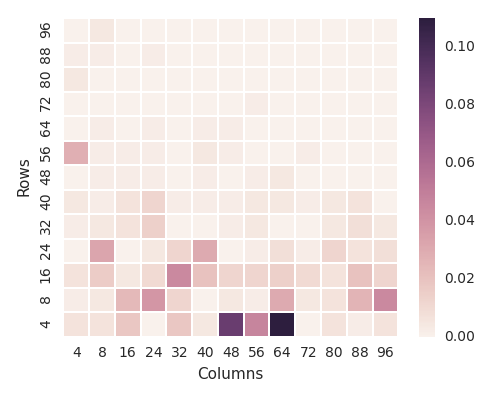
\includegraphics{gen/img/oracle_param_space.pdf}
\vspace{-1.5em} % Shrink vertical padding
\caption{}
\label{fig:oracle-wgsizes}
\end{subfigure}
\\
\begin{subfigure}[t]{0.98\textwidth}
\centering
\includegraphics{gen/img/coverage_space.pdf}
\vspace{-1.5em} % Shrink vertical padding
\caption{}
\label{fig:coverage}
\end{subfigure}
\caption[Workgroup size legality and optimality]{%
  Log frequency counts for: (\subref{fig:oracle-wgsizes}) optimality,
  and (\subref{fig:coverage}) legality for a subset of the aggregated
  workgroup size optimisation space, $w_c \le 100, w_r \le 100$. The
  space of oracle workgroup size frequencies is highly irregular and
  uneven, with a peak frequency of $w_{(64 \times 4)}$. Legality
  frequencies are highest for smaller row and column counts (where
  $w < W_{\max}(s) \forall s \in S$), and $w_c$ and $w_r$ values which
  are multiples of 8.%
}
\label{fig:heatmaps}
\end{figure}

As explained in Section~\ref{sec:op-params}, the space of legal
workgroup sizes $W_{legal}(s)$ for a given scenario $s$ comprises all
workgroup sizes which: do not exceed the maximum allowed by the OpenCL
device and kernel $W_{\max}(s)$, and are not refused by the OpenCL
runtime.

\subsubsection{Maximum workgroup sizes}

\begin{figure}
  \centering
  \includegraphics{gen/img/max_wgsizes.pdf}
  \vspace{-1.5em} % Shrink vertical padding
  \caption[Workgroup size coverage]{%
    A subset of the aggregated workgroup size optimisation space,
    $w_c \le 100, w_r \le 100$, showing the \emph{coverage} of each
    workgroup size, i.e.\ the ratio of scenarios for which a workgroup
    size satisfies architecture and kernel enforced constraints
    ($W_{\max}(s)$). Workgroup sizes with a coverage of $< 1$ fail to
    satisfy these constraints for one or more scenarios. Only
    workgroup sizes with a coverage of 1 may be used for static
    tuning, which greatly reduces the size of the optimisation
    space. Observed $W_{\max}(s)$ values are multiples of 256, hence
    the abrupt ``steps'' in coverage.%
  }
\label{fig:max-wgsizes}
\end{figure}

We define the \emph{coverage} of a workgroup size to be the ratio
$0 \le x \le 1$ between the number of scenarios for which the
workgroup size was less than $W_{\max}(s)$, normalised to the total
number of workgroup sizes. A coverage of 1 implies a workgroup size
which is always legal for all combinations of stencil and
architecture. A workgroup size with a coverage of 0 is never
legal. Figure~\ref{fig:max-wgsizes} plots the coverage of a subset of
the workgroup size optimisation space.

Note that since $W_{\max}(s)$ defines a hard limit for a given $s$, if
statically selecting a workgroup size, one must limit the optimisation
space to the smallest $W_{\max}(s)$ value, i.e.\ only the workgroup
sizes with a coverage of 1. The observed $W_{\max}(s)$ values range
from 256--8192, which results in up to a 97\% reduction in the size of
the optimisation space when $W_{\max}(s) = 8192$, even though only
14\% of scenarios have the minimum value of $W_{\max}(s) = 256$.

% Size of optimisation space for Wmax =  256: 273
% Size of optimisation space for Wmax = 8192: 15925

\subsubsection{Refused Parameters}

\begin{table}
\parbox{.32\linewidth}{
  \centering
  \scriptsize
  \rowcolors{2}{white}{gray!25}
  \input{gen/tab/top_refused_params_1}
}
\hfill
\parbox{.32\linewidth}{
  \centering
  \scriptsize
  \rowcolors{2}{white}{gray!25}
  \input{gen/tab/top_refused_params_2}
}
\hfill
\parbox{.32\linewidth}{
  \centering
  \scriptsize
  \rowcolors{2}{white}{gray!25}
  \input{gen/tab/top_refused_params_3}
}
\caption[Workgroup sizes most frequently refused]{%
  The thirty most refused parameters, ranked in descending
  order. There is little correlation between the size of workgroup and the
  likelihood that it is refused, suggesting that the cause of refused
  parameters is not a resource constraint, but a behavioural issue.%
}
\label{tab:top-refused-params}
\end{table}

\begin{figure}
\centering
\begin{subfigure}[h]{.45\textwidth}
  \centering
  \includegraphics{gen/img/refused_params_by_device}
  \caption{}
  \label{fig:refused-params-by-device}
\end{subfigure}
\hfill
\begin{subfigure}[h]{.45\textwidth}
  \centering
  \includegraphics{gen/img/refused_params_by_vendor}
  \caption{}
  \label{fig:refused-params-by-vendor}
\end{subfigure}
\caption[Refused workgroup sizes by device and vendor]{%
  The ratio of test cases with refused workgroup sizes, grouped by:
  (\subref{fig:refused-params-by-device}) OpenCL device ID;\
  (\subref{fig:refused-params-by-vendor}) device vendor ID. Parameters
  were refused most frequently by Intel i5 CPUs, then by
  previous-generation NVIDIA GPUs. No parameters were refused by AMD
  devices.%
}
\label{fig:refused-params-by-dev-vendor}
\end{figure}

In addition to the hard constraints imposed by the maximum workgroup
size, there are also refused parameters, which are workgroup sizes
which are rejected by the OpenCL runtime and do not provide a
functioning program. Of the 8504 unique workgroup sizes tested, 11.4\%
were refused in one or more test cases. An average of 5.5\% of all
test cases lead to refused parameters. For a workgroup size to be
refused, it must satisfy the architectural and program-specific
constraints which are exposed by OpenCL, but still lead to a
\texttt{CL\_OUT\_OF\_RESOURCES} error when the kernel is
enqueued. Table~\ref{tab:top-refused-params} lists the most frequently
refused parameters, and the percentage of test cases for which they
were refused. While uncommon, a refused parameter is an obvious
inconvenience to the user, as one would expect that any workgroup size
within the specified maximum should behave \emph{correctly}, if not
efficiently. Figure~\ref{fig:coverage} visualises the space of legal
workgroup sizes by showing the frequency counts that a workgroup size
is legal. Smaller workgroup sizes are legal most frequently due to the
$W_{\max}(s)$ constraints. Beyond that, workgroup sizes which contain
$w_c$ and $w_r$ values which are multiples of eight are more
frequently legal, which is a common width of SIMD vector
operations~\cite{IntelCorporation2012}.

Experimental results suggest that the problem is vendor --- or at
least device --- specific. By grouping the refused test cases by
device and vendor, we see a much greater quantity of refused
parameters for test cases on Intel CPU devices than any other type,
while no workgroup sizes were refused by the AMD
GPU. Figure~\ref{fig:refused-params-by-dev-vendor} shows these
groupings. The exact underlying cause for these refused parameters is
unknown, but can likely by explained by inconsistencies or errors in
specific OpenCL driver implementations.

As these OpenCL implementations are still in active development, it is
anticipated that errors caused by unexpected behaviour will become
more infrequent as the technology
matures. Figure~\ref{fig:refused-params-by-device} shows that the
ratio of refused parameters decreases across the three generations of
Nvidia GPUs: GTX 590 (2011), GTX 690 (2012), and GTX TITAN (2013). The
same is trend is apparent for the two Intel i5s: i5-2430M (2011), and
i5-4570 (2013), although not for the i7-3820 (2012). For now, it is
imperative that any autotuning system is capable of adapting to these
refused parameters by suggesting alternatives when they occur.


\subsection{Baseline Parameter}\label{subsec:baseline}

The baseline parameter $\bar{w}$ is the workgroup size which provides
the best overall performance while being legal for all scenarios. It
is the workgroup size $w \in W_{safe}$ which maximises the output of
the performance function $\bar{p}(w)$. As shown in
Table~\ref{tab:highest-legality}, only a \emph{single} workgroup size
$w_{(4 \times 4)}$ from the set of experimental results is found to
have a legality of 100\%, suggesting that an adaptive approach to
setting workgroup size is necessary not just for the sake of
maximising performance, but also for guaranteeing program correctness.

The utility of the baseline parameter is that it represents the best
performance that can be achieved through static tuning of the
workgroup size parameter. We can evaluate the performance of
suboptimal workgroup sizes by calculating the geometric mean of their
\emph{performance} for a particular scenario $p(s, w)$ across all
scenarios, $\bar{p}(w)$. The baseline parameter $\bar{p}(\bar{w})$
achieves only 24\% of the available
performance. Figure~\ref{fig:performance-legality} plots workgroup
size \emph{legality} and \emph{performance}, showing that there is no
clear correlation between the two. In fact, the workgroup sizes with
the highest mean performance are valid only for scenarios with the
largest $W_{\max}(s)$ value, which account for less than 1\% of all
scenarios, further reinforcing the case for adaptive tuning. The
workgroup sizes with the highest legality are listed in
Table~\ref{tab:highest-legality}, and the workgroup sizes with the
highest performance are listed in Table~\ref{tab:highest-performance}.

Figure~\ref{fig:speedups} shows the speedup of the oracle workgroup
size over the baseline parameter $w_{(4 \times 4)}$ for all
scenarios. If we assume that sufficiently pragmatic developer with
enough time would eventually find this static optimal, then this
provides a reasonable comparison for calculating speedups of an
autotuner for workgroup size. Comparing the runtime of workgroup sizes
relative to the oracle allows us to calculate upper bounds on the
possible performance which can be expected from autotuning.


\begin{figure}
\centering
\includegraphics{gen/img/params_summary.pdf}
\caption[Workgroup size legality vs.\ performance]{%
  Average legality and performance relative to the oracle of all
  workgroup sizes. Clearly, the relationship between legality and
  performance is not linear. Distinct vertical ``bands'' appear
  between regions of legality caused by the different $W_{\max}(s)$
  values of devices. The irregular jitter between these vertical bands
  is caused by refused parameters.%
}
\label{fig:performance-legality}
\end{figure}


\begin{table}
  \parbox{.45\linewidth}{
    \centering
    \scriptsize
    \rowcolors{2}{white}{gray!25}
    \input{gen/tab/top_params_coverage}
    \caption[Workgroup sizes with greatest legality]{%
      The 25 workgroup sizes with the greatest legality.%
    }
\label{tab:highest-legality}
  }
  \hfill
  \parbox{.45\linewidth}{
    \centering
    \scriptsize
    \rowcolors{2}{white}{gray!25}
    \input{gen/tab/top_params_perf}
    \caption[Workgroup sizes with greatest performance]{%
      The 25 workgroup sizes with the greatest mean
      performance.%
    }
\label{tab:highest-performance}
  }
\end{table}


\subsection{Speedup Upper Bounds}

\begin{figure}
  \includegraphics{gen/img/max_speedups}
  \caption[Workgroup size speedups]{%
    Speedup of oracle workgroup size over: the worst performing
    workgroup size for each scenario (\emph{Max}), the statically
    chosen workgroup size that provides the best overall performance
    ($w_{(4 \times 4)}$), and the human expert selected parameter
    ($w_{(32 \times 4)}$). Note that the human expert parameter is not
    legal for all scenarios.%
  }
\label{fig:speedups}
\end{figure}

For a given scenario $s$, the ratio of the workgroups sizes from
$W_{legal}(s)$ which provide the longest and shortest mean runtimes is
used to calculate an upper bound for the possible performance
influence of workgroup size:
%
\begin{equation}
r_{max}(s) = r(s, \argmax_{w \in W_{legal}(s)} t(s,w), \Omega(s))
\end{equation}
%
When applied to each scenario $s \in S$ of the experimental results,
we find the average of speedup upper bounds to be $15.14\times$ (min
$1.03\times$, max $207.72\times$). This demonstrates the importance of
tuning stencil workgroup sizes --- if chosen incorrectly, the runtime
of stencil programs can be extended by up to $207.72\times$. Note too
that for 5 of the scenarios, the speedup of the best over worst
workgroup sizes is $\le 5\%$.
% TODO: t-test for this!
For these scenarios, there is little benefit to autotuning; however,
this represents only 1.1\% of the tested scenarios. For 50\% of the
scenarios, the speedup of the best over worst workgroup sizes is
$\ge 6.19\times$.


\subsection{Human Expert}

% SCENARIOS IN WHICH 32x4 WAS NOT LEGAL:
%
% sqlite> select distinct name,kernels.north,kernels.south,kernels.east,kernels.west,device,dataset,name from runtime_stats left join scenarios on runtime_stats.scenario=scenarios.id left join kernel_names on scenarios.kernel=kernel_names.id left join kernels on scenarios.kernel=kernels.id where scenario NOT IN (select scenario from runtime_stats where params="32x4");
% name        north       south       east        west        device                                     dataset                name
% ----------  ----------  ----------  ----------  ----------  -----------------------------------------  ---------------------  ----------
% complex     30          30          30          30          1xIntel(R) Core(TM) i5-4570 CPU @ 3.20GHz  1024.1024.float.float  complex
% simple      0           0           0           0           1xIntel(R) Core(TM) i5-2430M CPU @ 2.40GH  1024.1024.float.float  simple
% complex     30          30          30          30          1xIntel(R) Core(TM) i5-2430M CPU @ 2.40GH  2048.2048.float.float  complex
% complex     1           10          30          30          1xIntel(R) Core(TM) i5-4570 CPU @ 3.20GHz  512.512.float.float    complex
% simple      30          30          30          30          1xIntel(R) Core(TM) i5-2430M CPU @ 2.40GH  512.512.float.float    simple
% complex     30          30          30          30          1xGeForce GTX 690                          512.512.float.float    complex
% simple      20          10          20          10          1xIntel(R) Core(TM) i5-2430M CPU @ 2.40GH  4096.4096.float.float  simple
% simple      1           10          30          30          1xIntel(R) Core(TM) i5-2430M CPU @ 2.40GH  2048.2048.float.float  simple
% complex     30          30          30          30          1xGeForce GTX 690                          1024.1024.float.float  complex
% complex     1           10          30          30          1xIntel(R) Core(TM) i5-2430M CPU @ 2.40GH  2048.2048.float.float  complex
% simple      30          30          30          30          1xGeForce GTX 690                          512.512.float.float    simple

In the original implementation of the SkelCL stencil
skeleton~\cite{Breuer2013}, \citeauthor{Breuer2013} selected a
workgroup size of $w_{(32 \times 4)}$ in an evaluation of 4 stencil
operations on a Tesla S1070 system. We can use this as an additional
parameter to compare the relative performance of workgroup sizes
against. However, the $w_{(32 \times 4)}$ workgroup size is invalid
for 2.6\% of scenarios, as it is refused in 11 test cases. By device,
those are: 3 on the GTX 690, 6 on the i5-2430M, and 2 on the i5-4570.
For the scenarios where $w_{(32 \times 4)}$ \emph{is} legal, the human
expert chosen workgroup size achieves an impressive geometric mean of
79.2\% of the oracle performance. The average speedup of oracle
workgroup sizes over the workgroup size selected by a human expert is
$1.37\times$ (min $1.0\times$, max $5.17\times$). Since the workgroup
size selected by the human expert is not legal for all scenarios, we
will examine the effectiveness of heuristics for tuning workgroup
size.


\subsection{Heuristics}\label{subsec:heuristics}

In this section we will consider the effectiveness of instead
selecting workgroup size using two types of heuristics. The first,
using the maximum workgroup size returned by the OpenCL device and
kernel APIs to select the workgroup size adaptively. The second, using
per-device heuristics, in which the workgroup size is selected based
on the specific architecture that a stencil is operating on.

\subsubsection{Using maximum legal size}

A common approach taken by OpenCL developers is to set the workgroup
size for a kernel based on the maximum legal workgroup size queried
from the OpenCL APIs. For example, to set the size of 2D workgroup, a
developer the square root of the (scalar) maximum wgsize to set the
number of columns and rows (since $w_c \cdot w_r$ must be
$< W_{\max}(s)$). To consider the effectiveness of this approach, we
group the workgroup size performances based on the ratio of the
maximum allowed for each scenario. We can also perform this for each
of the two dimensions --- rows and columns --- of the stencil
workgroup size.

Figure~\ref{fig:performance-wgsizes} shows the distribution of
runtimes when grouped this way, demonstrating that the performance of
(legal) workgroup sizes are not correlated with the maximum workgroup
sizes $W_{\max}(s)$. However, when considering individual components,
we observe that the best median workgroup size performances are
achieved with a number of columns that is between 10\% and 20\% of the
maximum, and a number of rows that is between 0\% and 10\% of the
maximum.

\subsubsection{Per-device workgroup sizes}

\begin{table}
\scriptsize
\centering
\rowcolors{2}{white}{gray!25}
\input{gen/tab/heuristics-dev}
\caption[Performance of tuning with a per-device heuristic]{%
  Selecting workgroup size using a per-device heuristic. The mode
  optimal workgroup size for each device type $\bar{w}$ is evaluated
  based on legality, and relative performance to the oracle (minimum
  and average) when legal.%
}
\label{tab:heuristic-dev}
\end{table}

One possible technique to selecting workgroup size is to tune
particular values for each targeted execution device. This approach is
sometimes adopted for cases with particularly high requirements for
performance on a single platform, so it produces an interesting
contrast to evaluating a machine learning approach, which attempts to
predict workgroup sizes for unseen platforms without the need for an
expensive exploration phase on the new platform.

Figure~\ref{fig:performances} shows the performance of workgroup sizes
relative to the oracle across scenarios grouped by: kernel, device,
and dataset. When grouped like this, a number of observations can
made. First is that not all of the kernels are sensitive to tuning
workgroup size to the same degree. The \emph{sobel} kernel has the
lowest median performance, indicating that it is the most profitable
to tune, while the \emph{threshold} kernel is the least
profitable. Similarly, the Intel i7-3820 is far less amenable to
tuning than the other devices, while the Intel i5-4570 is the most
sensitive to the workgroup size parameter. Such variances in the
distributions of workgroup sizes suggest that properties underlying
the architecture, kernel, and dataset all contribute towards the
proper selection of workgroup size.

To test the performance of a per-device heuristic for selecting
workgroup size, we group the scenarios by device, and compare the
relative performance of all workgroup sizes for each group of
scenarios. The most frequently optimal workgroup size $\bar{w}$ for
each device is selected, and the legality and performance of each
scenario using that workgroup size is evaluated.
Table~\ref{tab:heuristic-dev} shows the results of this evaluation.
The GTX 690 and GTX TITAN share the same $\bar{w}_{(64 \times 4)}$
value, while every other device has a unique optimum. The general case
performance of these per-device parameters is very good, although
legality is only assured for the GTX TITAN and AMD 7970 (which did not
refuse any parameters). However, the worst case performance of
per-device workgroup sizes is poor for all except the i7-3820 (which
is least sensitive to tuning), suggesting that device alone is not
capable of reliably informing the choice of workgroup size.


\begin{figure}
\begin{subfigure}[h]{\textwidth}
\centering
\includegraphics{gen/img/performance_max_wgsize}
\vspace{-1.5em} % Shrink vertical padding
\caption{}
\label{fig:performance-max-wgsize}
\end{subfigure}
\\
\begin{subfigure}[h]{.48\textwidth}
\centering
\includegraphics{gen/img/performance_max_c}
\vspace{-1.5em} % Shrink vertical padding
\caption{}
\label{fig:performance-wg-c}
\end{subfigure}
~%
\begin{subfigure}[h]{.48\textwidth}
\centering
\includegraphics{gen/img/performance_max_r}
\vspace{-1.5em} % Shrink vertical padding
\caption{}
\label{fig:performance-wg-r}
\end{subfigure}

\caption[Workgroup size performances vs.\ size]{%
  Comparing workgroup performance relative to the oracle as function
  of: (\subref{fig:performance-max-wgsize})~maximum legal size,
  (\subref{fig:performance-wg-c})~number of columns, and
  (\subref{fig:performance-wg-r})~ number of rows. Each workgroup
  size is normalised to the maximum allowed for that scenario, $W_{\max}(s)$.%
}
\label{fig:performance-wgsizes}
\end{figure}
\newpage
\begin{figure}t
\begin{subfigure}[h]{\textwidth}
\centering
\includegraphics{gen/img/performance_kernels.pdf}
\vspace{-1.5em} % Shrink vertical padding
\caption{Kernels}
\label{fig:performance-kernels}
\end{subfigure}
\\
\begin{subfigure}[h]{.48\textwidth}
\centering
\includegraphics{gen/img/performance_devices.pdf}
\vspace{-1.5em} % Shrink vertical padding
\caption{Devices}
\label{fig:performance-devices}
\end{subfigure}
~%
\begin{subfigure}[h]{.48\textwidth}
\centering
\includegraphics{gen/img/performance_datasets.pdf}
\vspace{-1.5em} % Shrink vertical padding
\caption{Datasets}
\label{fig:performance-datasets}
\end{subfigure}

\caption[Workgroup size performances across device, kernel, and dataset]{%
  Performance relative to the oracle of workgroup sizes across all
  test cases, grouped by: (\subref{fig:performance-kernels})~kernels,
  (\subref{fig:performance-devices})~devices, and
  (\subref{fig:performance-datasets})~datasets.%
}
\label{fig:performances}
\end{figure}


\subsection{Summary}

In this section we have explored the performance impact of the
workgroup size optimisation space. By comparing the relative
performance of an average of 629 workgroup sizes for each of 429
scenarios, the following conclusions can be drawn:

\begin{enumerate}
\item The performance of a workgroup size for a particular scenario
  depends properties of the hardware, software, and dataset.
\item The performance gap between the best and workgroup sizes for a
  particular combination of hardware, software, and dataset is up to
  $207.72\times$.
\item Not all workgroup sizes are legal, and the space of legal
  workgroup sizes cannot statically be determined. Adaptive tuning of
  workgroup size is required to ensure reliable performance.
\item Differing scenarios have wildly different optimal workgroup
  sizes, and the best performance can be achieved using static tuning
  is optimal for only 15\% of scenarios.
\end{enumerate}
%
% I believe this presents a compelling case for the development of an
% autotuner which can select the optimal workgroup size at runtime.
%
In the following section, we will evaluate the performance of OmniTune
for selecting workgroup sizes.


\section{Autotuning Workgroup Sizes}

In this section, we evaluate the performance of OmniTune for
predicting workgroup sizes of SkelCL skeletons, using the prediction
techniques described in Section~\ref{sec:omnitune-ml}. For each
technique, we partition the experimental data into training and
testing sets, $S_{training} \subset S$ and
$S_{testing} = S - S_{training}$. A set of labelled training data
$D_{training}$ is derived from $S_{training}$, and the prediction
quality is testing using the validation set $D_{testing}$ derived from
$S_{training}$. We use multiple approaches to partitioning test data,
to evaluate the prediction quality under different scenarios. The
processes for generating validation sets are:
%
\begin{itemize}
\item 10-fold --- shuffle the set of all training and divide into 10
  validation sets, each containing 10\% of the training data. This
  process is repeated for 10 rounds, resulting in 100 validations.
\item Synthetic --- divide the training data such that it consists
  solely of data collected from synthetic benchmarks, and use data
  collected from real-world benchmarks to test.
\item Device --- partition the training data into $n$ sets, one for
  each device. Use $n-1$ sets for training, repeating until partition
  has been used for testing.
\item Kernel --- partition the training data into $n$ sets, one for
  each kernel. Use $n-1$ sets for training, repeating until partition
  has been used for testing.
\item Dataset --- partition the training data into $n$ sets, one for
  each type of dataset. Use $n-1$ sets for training, repeating until
  partition has been used for testing.
\end{itemize}
%
For each autotuning technique, the results of testing using the
different validation set are reported separately. The autotuning
techniques evaluated are: using classifiers to predict the optimal
workgroup size of a stencil, with fallback strategies to handle
illegal predictions; using regressors to predict the runtime of a
stencil using different workgroup sizes, and selecting the legal
workgroup size which has the lowest predicted runtime; and using
regressors to predict the relative performance of workgroup sizes over
a baseline, and selecting the workgroup size which has the highest
predicted relative performance. We first describe the evaluation
strategies for each technique, before presenting experimental results
and analysis.


\subsection{Evaluating Classifiers}

The methodology for selecting workgroup size using classifiers is
described in Section~\ref{subsec:omnitune-ml-class}. Training data
consists of pairs of feature vectors $f(s)$ and oracle workgroup sizes
$\Omega(s)$:
%
\begin{equation}
  D_{training} = \left\{ (f(s),\Omega(s)) | s \in S_{training} \right\}
\end{equation}
%
Testing data are not labelled with oracle workgroup sizes:
%
\begin{equation}
  D_{testing} = \left\{ f(s) | s \in S_{testing} \right\}
\end{equation}
%
Each classifier is evaluated using the three different classification
techniques: \textsc{Baseline}, \textsc{Random}, and
\textsc{NearestNeighbour}, which differ in the way in which they
handle illegal predictions. Illegal predictions occur either because
the classifier has suggested a parameter which does not satisfy the
maximum workgroup size constraints $w > W_{\max}(s)$, or because the
workgroup size is refused by OpenCL $w \in W_{refused}(s)$. Workgroup
sizes are predicted for each scenario in the testing set, and the
quality of the predicted workgroup size is evaluated using the
following metrics:
%
\begin{itemize}
\item accuracy (binary) --- whether the predicted workgroup size is
  the true oracle, $p(f(s)) = \Omega(s)$.
\item validity (binary) --- whether the classifier predicted a
  workgroup size which satisfies the workgroup size constraints
  constraints, $p(f(s)) < W_{\max}(s)$.
\item refused (binary) --- whether the classifier predicted a
  workgroup size which is refused, $p(f(s)) \in W_{refused}(s)$.
\item performance (real) --- the relative performance of the predicted
  workgroup size relative to the oracle,
  $0 \le r(p(f(s)), \Omega(s)) \le 1$.
\item speedups (real) --- the relative performance of the predicted
  workgroup size relative to the baseline workgroup size
  $w_{(4 \times 4)}$, and human expert workgroup size
  $w_{(32 \times 4)}$ (where applicable).
\item time (real) --- the round trip required to make the prediction,
  as measured by the OmniTune client. This includes classification
  time and inter-process communication overheads between the client
  and server.
\end{itemize}
%
The \emph{validty} and \emph{refused} metrics measure how often
fallback strategies are required to select a legal workgroup size
$w \in W_{legal}(s)$.


\subsection{Evaluating Regressors}

Sections~\ref{subsec:omnitune-ml-runtime}
and~\ref{subsec:omnitune-ml-speedup} describe methodologies for
selecting workgroup sizes by predicting program runtimes or relative
performance, respectively. The evaluation approach for both
methodologies is the same, only the training data differs. For
predicting runtimes, training data consists of feature vectors,
labelled with the mean observed runtime $t(s,w)$ for all legal
workgroup sizes:
%
\begin{equation}
  D_{training} = \bigcup_{\forall s \in S_{training}} \left\{ (f(s),t(s,w)) | w \in W_{legal}(s)
  \right\}
\end{equation}
For predicting speedups, the features vectors are labelled with
observed speedup over the baseline parameter $\bar{w}$ (see
Section~\ref{subsec:baseline}) for all legal workgroup sizes:
\begin{equation}
  D_{training} = \cup \left\{ (f(s),r(s,w,\bar{w})) | w \in W_{legal}(s)
  \right\} \forall s \in S_{training}
\end{equation}
%
Test data consists of unlabelled feature vectors:
%
\begin{equation}
  D_{testing} = \left\{ f(s) | s \in S_{testing} \right\}
\end{equation}
%
The quality of predicted workgroup sizes is evaluated using the
following metrics:
%
\begin{itemize}
\item accuracy (binary) --- whether the predicted workgroup size is
  the true oracle, $p(f(s)) = \Omega(s)$.
\item performance (real) --- the relative performance of the predicted
  workgroup size relative to the oracle,
  $0 \le r(p(f(s)), \Omega(s)) \le 1$.
\item speedups (real) --- the relative performance of the predicted
  workgroup size relative to the baseline workgroup size
  $w_{(4 \times 4)}$, and human expert workgroup size
  $w_{(32 \times 4)}$ (where applicable).
\item time (real) --- the round trip required to make the prediction,
  as measured by the OmniTune client. This includes classification
  time and inter-process communication overheads between the client
  and server.
\end{itemize}
%
Unlike with classifiers, the process of selecting workgroup sizes
using regressors is resistant to refused parameters, so no fallback
strategies are required, and the \emph{validity} and \emph{refused}
metrics are not used.


\subsection{Results and Analysis}

The purpose of this evaluation is to test the effectiveness of machine
learning-enabled autotuning for predicting workgroup sizes of SkelCL
stencils codes. First, we consider the prediction performance of
classifiers.


% \cleardoublepage
\begin{figure}
\centering
\includegraphics{gen/img/classification-syn-real}
\caption[Classification results using synthetic benchmarks]{%
  Classification results for synthetic benchmarks. Each classifier is
  trained on data from synthetic stencils, and tested for prediction
  quality using data from 6 real world benchmarks.%
}
\label{fig:class-syn}
\end{figure}
\newpage
\begin{figure}
\centering
\includegraphics{gen/img/classification-arch}
\caption[Classification results using cross-device evaluation]{%
  Classification results of cross-device evaluation. Each classifier
  is trained using data from $n-1$ devices, and tested for prediction
  quality using data for the $n^{th}$ device.%
}
\label{fig:class-arch}
\end{figure}
\begin{figure}
\centering
\begin{subfigure}[h]{.45\textwidth}
\centering
\includegraphics{gen/img/runtime-class-xval}
\caption{}
\label{fig:runtime-class-xval}
\end{subfigure}
~%
\begin{subfigure}[h]{.45\textwidth}
\centering
\includegraphics{gen/img/speedup-class-xval}
\caption{}
\label{fig:speedup-class-xval}
\end{subfigure}
\caption[Autotuning performance using regressors]{%
  Evaluating the effectiveness of classification using regressors, by
  predicting: (\subref{fig:runtime-class-xval}) the workgroup size
  with the minimal runtime, and (\subref{fig:speedup-class-xval}) the
  workgroup size with the greatest speedup over a baseline.%
}
\label{fig:regression-class}
\end{figure}

With the exception of the ZeroR, which predicts \emph{only} the
baseline workgroup size $w_{\left( 4 \times 4 \right)}$, the
classifiers achieve good speedups over the baseline. Average
classification speedups across all validations range between
$4.61\times$ and $5.05\times$. Figures~\ref{fig:class-syn}
and~\ref{fig:class-arch} show a summary of results using 10-fold
cross-validation and cross-device validation, respectively.  The
highest average speedup is achieved by SMO, and the lowest by Naive
Bayes. The difference between average speedups is not significant
between the types of classifier, with the exception of SimpleLogistic,
which performs poorly when trained with synthetic benchmarks and
tested against real-world programs. This suggests the model
over-fitting to features of the synthetic benchmarks which are not
shared by the real-world
tests. Figure~\ref{fig:classification-speedups} shows the distribution
of predictions speedups for each prediction technique.

\begin{figure}
\centering
\includegraphics{gen/img/fallback_speedups}
\caption[Comparison of fallback handler speedups]{%
  Comparison of fallback handlers, showing the speedup over baseline
  parameter for all test cases where a classifier predicted an illegal
  workgroup size.%
}
\label{fig:fallback-speedups}
\end{figure}

By isolating the test cases where classifiers predicted an illegal or
refused parameter, we can directly compare the relative effectiveness
of each fallback handler. The fallback handler with the best average
case performance is \textsc{NearestNeighbour}, with an average speedup
across all classifiers and validation sets of $5.26\times$. The
speedup of \textsc{Random} fallback handler is $3.69\times$, and
$1.0\times$ for \textsc{Baseline}. Figure~\ref{fig:fallback-speedups}
plots the speedups of each fallback handler for all of these isolated
test cases. Interestingly, both the lowest and highest speedups are
achieved by the \textsc{Random} fallback handler, since it essentially
performs a random exploration of the optimisation space. However, the
\textsc{NearestNeighbour} fallback handler provides consistently
greater speedups for the majority of test cases, indicating that it
successfully exploits the structure of the optimisation spaces.

Figures~\ref{fig:runtime-class-xval} and ~\ref{fig:speedup-class-xval}
show a summary of results for classification using regressors to
predict program runtimes and speedups, respectively. Of the two
regression techniques, predicting the \emph{speedup} of workgroup
sizes is much more successful than predicting the \emph{runtime}. This
is most likely caused by the inherent difficulty in predicting the
runtime of arbitrary programs, where dynamic factors such as flow
control and loop bounds are not captured by the kernel features used
in OmniTune, which instead use simple static static instruction counts
and densities. The average speedup achieved by predicting runtimes is
$4.14\times$. For predicting speedups, the average is $5.57\times$.
Tables~\ref{tab:class}, \ref{tab:runtime-class},
and~\ref{tab:speedup-class} show mean performances and speedups for:
J48 classifier using the \textsc{NearestNeighour} fallback strategy,
classification using runtime regression, and classification using
speedup regression, respectively.

If we eliminate the 2.6\% of test cases for which the workgroup size
of $w_{(32 \times 4)}$ is illegal, we can compare the performance of
OmniTune directly against the human expert chosen workgroup
size. Figure~\ref{fig:speedup-distributions} compares the speedups of
all such validation instances over the human expert parameter, for
each autotuning technique. The speedup distributions show consistent
classification results for the five classification techniques, with
the speedup at the lower quartile for all classifiers being
$\ge 1.0\times$. The IQR for all classifiers is $< 0.5$, but there are
outliers with speedups both well below $1.0\times$ and well above
$2.0\times$. In contrast, the speedups achieved using runtime
regression have a lower range, but also a lower median and a larger
IQR. Clearly, runtime regression is the least effective of the
evaluated autotuning techniques.

% The lower average speedup attained by speedup regression over the
% J48 classifier belies the fact that the \emph{median} speedup is
% much greater, at $1.33 \times$.


\begin{figure}
\centering
\includegraphics{gen/img/speedup-distributions}
\caption[Speedup results over human expert]{%
  Distributions of speedups over \emph{human expert}, ignoring cases
  where human expert prediction is invalid. Classifiers are using
  \textsc{NearestNeighbour} fallback handlers. The speedup axis is
  fixed to the range 0--2.5 to highlight the IQRs, which results in
  some outliers > 2.5 being clipped.%
}
\label{fig:speedup-distributions}
\end{figure}





\begin{table}
\scriptsize
\centering
\rowcolors{2}{white}{gray!25}
\input{gen/tab/class}
\caption{Validation results for J48 and \textsc{NearestNeighbour}
  classification.}
\label{tab:class}
\end{table}
\begin{table}
\scriptsize
\centering
\rowcolors{2}{white}{gray!25}
\input{gen/tab/class-runtime}
\caption{Validation results for runtime regression.}
\label{tab:runtime-class}
\end{table}
\begin{table}
\scriptsize
\centering
\rowcolors{2}{white}{gray!25}
\input{gen/tab/class-speedup}
\caption{Validation results for speedup regression.}
\label{tab:speedup-class}
\end{table}


% \subsection{Visualising Prediction Errors}

\begin{figure}
\centering
\begin{subfigure}[t]{0.45\textwidth}
\centering
\includegraphics{gen/img/heatmap_1}
\vspace{-1.5em} % Shrink vertical padding
\caption{}
\label{fig:class-hmaps-1}
\end{subfigure}
~%
\begin{subfigure}[t]{0.45\textwidth}
\centering
\includegraphics{gen/img/heatmap_2}
\vspace{-1.5em} % Shrink vertical padding
\caption{}
\label{fig:class-hmaps-2}
\end{subfigure}
\\
\begin{subfigure}[t]{0.45\textwidth}
\centering
\includegraphics{gen/img/heatmap_3}
\vspace{-1.5em} % Shrink vertical padding
\caption{}
\label{fig:class-hmaps-3}
\end{subfigure}
~%
\begin{subfigure}[t]{0.45\textwidth}
\centering
\includegraphics{gen/img/heatmap_5}
\vspace{-1.5em} % Shrink vertical padding
\caption{}
\label{fig:class-hmaps-4}
\end{subfigure}
\\
\begin{subfigure}[t]{0.45\textwidth}
\centering
\includegraphics{gen/img/reg_runtime_heatmap}
\vspace{-1.5em} % Shrink vertical padding
\caption{}
\label{fig:class-hmaps-5}
\end{subfigure}
~%
\begin{subfigure}[t]{0.45\textwidth}
\centering
\includegraphics{gen/img/reg_speedup_heatmap}
\vspace{-1.5em} % Shrink vertical padding
\caption{}
\label{fig:class-hmaps-6}
\end{subfigure}
\caption[Prediction errors across classification techniques]{%
  Heatmaps of classification errors for 10-fold cross-validation,
  showing a subset of the optimisation space. The shading in each
  cells indicates if it is predicted less frequently (blue), ore more
  frequently (red) than it is optimal. Colour gradients are normalised
  across plots.%
}
\label{fig:class-hmaps}
\end{figure}


Only the NaiveBayes and RandomForest classifiers predicted the human
expert selected workgroup size of $w_{(32 \times 4)}$ as frequently,
or more frequently, than it was optimal.

% \subsection{Autotuning Costs}\label{subsec:autotune-costs}

Prediction costs using regression are significantly greater than using
classifiers. This is because, while a classifier makes a single
prediction, the number of predictions required of a regressor grows
with the size of $W_{\max}(s)$, since classification with regression
requires making predictions for all
$w \in \left\{ w | w < W_{\max}(s) \right\}$.

\TODO{What is the costs of autotuning?}

\TODO{How many iterations do we need to do before we ``break even''?}


\subsection{Summary}

From an evaluation of 17 different autotuning techniques using 5
different types of validation sets, the following conclusions about
autotuning performance can be drawn:
%
\begin{itemize}
\item In the case of classifiers predicting illegal workgroup sizes,
  the best fallback strategy is to select the closest legal workgroup
  size.
\item The performance of predicted workgroup sizes for unseen devices
  is within 8\% of the performance for known devices.
\item Predicting the \emph{runtime} of stencils is the least effective
  of the evaluated autotuning techniques, achieving an average of only
  68\% of the available performance.
\item Classification using regression costs an order of magnitude more
  time than using classifiers. The J48 classifier has the lowest
  overhead.
\end{itemize}
%

% \section{Summary}


\section{Conclusions}\label{sec:conclusions}
\section{Critical Analysis}

\section{Future Work}

% TODO: Extensions to SkelCL: Cluster parallelism, multi-dimensional
% stencils, stencil specialisations for specific memory access
% patterns.

% TODO: Additional optimisation parameters, e.g. which device to
% execute on.

% TODO: Apply to additional skeleton libraries.

% TODO: energy as an optimisation cotarget.


% Leather, H., O’Boyle, M., & Worton, B. (2009). Raced Profiles:
% Efficient Selection of Competing Compiler Optimizations. In LCTES
% ’09: Proceedings of the ACM SIGPLAN/SIGBED 2009 Conference on
% Languages, Compilers, and Tools for Embedded Systems
% (pp. 1–10). Dublin.
\TODO{%
  Consider using adaptive sampling plans and some sort of global
  mechanism for performing cooperative exploration across multiple
  devices, while reducing the number of samples required to
  distinguish good from bad workgroup sizes~\cite{Leather2009}.%
}

\TODO{%
  Make the remote active. Rather than simply fetching from remote SQL
  tables, the remote could be a webserver with a REST api for HTTP
  GET/PUT of training data, and could analyse the data and build
  models asynchronously.%
}


\label{bibliography}
\printbibliography

\end{document}

